\documentclass[a4paper,14pt]{extarticle}
\usepackage{geometry}
\usepackage[T1]{fontenc}
\usepackage[utf8]{inputenc}
\usepackage[english,russian]{babel}
\usepackage{amsmath}
\usepackage{amsthm}
\usepackage{amssymb}
\usepackage{fancyhdr}
\usepackage{setspace}
\usepackage{graphicx}
\usepackage{colortbl}
\usepackage{tikz}
\usepackage{pgf}
\usepackage{subcaption}
\usepackage{listings}
\usepackage{indentfirst}
\usepackage[colorlinks,citecolor=blue,linkcolor=blue,bookmarks=false,hypertexnames=true, urlcolor=blue]{hyperref} 
\usepackage{indentfirst}
\usepackage{mathtools}
\usepackage{booktabs}
\usepackage[flushleft]{threeparttable}
\usepackage{tablefootnote}
\usepackage{multirow}

\usepackage{chngcntr} % нумерация графиков и таблиц по секциям
\counterwithin{table}{section}
\counterwithin{figure}{section}

\graphicspath{{graphics/}}%путь к рисункам

\makeatletter
\renewcommand{\@biblabel}[1]{#1.} % Заменяем библиографию с квадратных скобок на точку:
\makeatother

\geometry{left=2.5cm}% левое поле
\geometry{right=1.5cm}% правое поле
\geometry{top=1.5cm}% верхнее поле
\geometry{bottom=1.5cm}% нижнее поле
\renewcommand{\baselinestretch}{1.5} % междустрочный интервал


\newcommand{\bibref}[3]{\hyperlink{#1}{#2 (#3)}} % biblabel, authors, year
\addto\captionsrussian{\def\refname{Список литературы (или источников)}} 

\renewcommand{\theenumi}{\arabic{enumi}}% Меняем везде перечисления на цифра.цифра
\renewcommand{\labelenumi}{\arabic{enumi}}% Меняем везде перечисления на цифра.цифра
\renewcommand{\theenumii}{.\arabic{enumii}}% Меняем везде перечисления на цифра.цифра
\renewcommand{\labelenumii}{\arabic{enumi}.\arabic{enumii}.}% Меняем везде перечисления на цифра.цифра
\renewcommand{\theenumiii}{.\arabic{enumiii}}% Меняем везде перечисления на цифра.цифра
\renewcommand{\labelenumiii}{\arabic{enumi}.\arabic{enumii}.\arabic{enumiii}.}% Меняем везде перечисления на цифра.цифра

\begin{document}
\begin{titlepage}
\newpage

{\setstretch{1.0}
\begin{center}
Федеральное государственное автономное образовательное учреждение высшего образования «Национальный исследовательский университет «Высшая школа экономики»
\\
\bigskip
Факультет компьютерных наук \\
Основная образовательная программа \\
Прикладная математика и информатика \\
\end{center}
}

\vspace{8em}

\begin{center}
{\Large КУРСОВАЯ РАБОТА}\\
\textsc{\textbf{
Исследовательский проект на тему
\linebreak
"Прогнозирование временных рядов с помощью динамических авторегрессионных моделей"}}
\end{center}

\vspace{2em}

{\setstretch{1.0}
\hfill\parbox{16cm}{
\hspace*{5cm}\hspace*{-5cm}Выполнил студент группы 192, 3 курса,\\
 Лоптев Сергей Евгеньевич\\
 
\hspace*{5cm}\hspace*{-5cm}Руководитель КР:\\
научный сотрудник Зехов Матвей Сергеевич\\

%\hspace*{5cm}\hspace*{-5cm}Куратор:\hfill < степень>, <звание>, <ФИО полностью>\\

}
}

\vspace{\fill}

\begin{center}
Москва 2022
\end{center}

\end{titlepage}% это титульный лист
\newpage

{
	\hypersetup{linkcolor=black}
	\tableofcontents
}

\newpage
\section*{Аннотация}
Существует множество популярных моделей, используемых в прогнозировании временных рядов. В данной работе мы реализуем не самые популярные модели --- \textit{динамические авторегрессионные модели}. Мы статистически сравниваем данные модели с базовыми моделями --- ARIMA, ETS, PROPHET и наивной на выборке M4. Кроме обычной динамической регрессии вводится динамическая регрессия с сезонностью; для неё также проводится статистическое сравнение. Кроме того, проводится исследование особенностей временных рядов, на которых динамические модели выдают лучшее качество. Мы показываем, что динамические модели в целом не хуже, чем базовые методы, работают в прогнозировании временных рядов. При этом на качество работы динамических моделей может влиять периодичность временного ряда, сезонность и горизонт прогнозирования.

\textit{Ключевые слова: динамическая регрессия, DLS, динамические наименьшие квадраты, ETS, ARIMA, PROPHET, наивная модель, временные ряды, прогнозирование временных рядов.}

There are a lot of popular models in time series forecasting. In this paperwork we implement not so popular \textit{dynamic autoregression models}. We conduct statistical comparison with baselines: ARIMA, ETS, PROPHET and naive models on the M4 dataset.  Apart from dynamic regression we implement dynamic regression with seasonality; we conduct statistical tests for it as well. We show that dynamic models generally have a worse performance than the baseline. At the same time, periodicity and seasonality of time series may influence quality of dynamic models predicts, as well as forecasting horizon.

\textit{Keywords: dynamic regression, DLS, dynamic least squares, ETS, ARIMA, PROPHET, naive model, time series, time series forecasting.}

\section{Введение}
Прогнозирование временных рядов — это достаточно часто встречаемая в индустрии задача. Она решается, например, в финансах, бизнесе и IT, причём свойства прогнозируемых рядов сильно варьируются. Задача прогнозирования временного ряда зачастую сводится к перебору известных моделей и подбору гиперпараметров. В этой статье мы сравним работу динамических регрессионных моделей с такими моделями, как ETS, ARIMA, PROPHET, наивная модель на большом количестве реальных временных рядов. Кроме того, мы классифицируем ряды, на которых динамическая регрессия показывает себя лучше остальных моделей. Таким образом, задача бьётся на несколько конкретных подзадач: оптимальная реализация градиентного спуска для динамических моделей на языках Python и C++, применение динамических и описанных выше моделей на большом количестве реальных временных рядов, и оценка полученных результатов.

Динамические регрессионные модели были достаточно детально изучены теоретически. Например, были выведены свойства оценок параметров с помощью динамического метода, а также проводилось сравнение динамических моделей с обычной линейной регрессией на синтетических данных (\bibref{hartley72}{Hartley M. J.}{1972}, \bibref{johnston74}{Johnston et al.}{1974}). В последнее время было выпущено несколько статей с реализацией динамических моделей (\bibref{gandrud15}{Gandrud, C. et al.}{2015}, \bibref{williams11}{Williams, L. K., Whitten, G. D.}{2011}), но все они имеют свои недостатки с точки зрения задачи, которую мы ставим. Таким образом, наша постановка задачи имеет практическую ценность, так как все работы о данной модели рассматривали её в основном именно в теоретическом ключе.

В результате проведения работы мы получили, что динамические модели в целом справляются с предсказанием не хуже, чем остальные представленные модели. Мы делили ряды на кластеры по периодичности, источнику, сезонности и стационарности; в среднем по каждому признаку процент побед динамической регрессии (то есть, лучшая MAE, чем у остальных моделей) составляет около 20-30\%. С точки зрения классификации рядов можно сделать вывод, что периодичность и сезонность ряда могут влиять на качество динамических моделей относительно базовых методов. Кроме того, было сделано наблюдение о том, что ошибка динамических моделей относительно базовых методов больше на многошаговом прогнозе (то есть, на дальний шаг), чем на одношаговом, и ещё больше, если мы пытаемся прогнозировать весь путь до этого дальнего шага.

Код работы доступен по ссылке \href{https://github.com/beastSL/coursework-3}{\texttt{https://github.com/beastSL/coursework-3}}.

\section{Обзор литературы}
Как уже было упомянуто, мы собираемся сравнивать новый метод с базовыми методами. Коротко опишем их.
\begin{itemize}
	\item ARIMA (и метод её оценки) была представлена в \bibref{box70}{Box G., Jenkins G.}{1970}. Эта модель — улучшение модели ARMA, позволяющее эффективно прогнозировать нестационарные (с точки зрения тренда) ряды. Компонента AR (AutoRegressive) названия означает, что в качестве регрессоров мы используем лагированные значения ряда; компонента I (Integrated) означает, что вместо сырых значений ряда мы возьмём разности соседних значений, возможно, несколько раз, компонента MA означает, что целевая переменная линейно зависит от ошибок за прошлые моменты времени. Модель ARIMA имеет три гиперпараметра $p$, $d$ и $q$, и представляет собой следующую формулу:
	\begin{equation*}
		\triangle^{d} y_t = c + \sum_{i=1}^p a_i \triangle^d y_{t-i} + \sum_{j=1}^q b_j \varepsilon_{t-j} + \varepsilon_t.
	\end{equation*}
	\item ETS --- модель, представленная в \bibref{brown56}{Brown R. G.}{1956} и улучшенная и расширенная в \bibref{holt57}{Holt C. C.}{1957}. В самом базовом виде ETS задаётся следующими уравнениями:
	\begin{align*}
		&\hat{y}_1 = y_0 \\
		&\hat{y}_t = \alpha y_{t-1} + (1 - \alpha \hat{y}_{t-1}) = \hat{y}_{t-1} + \alpha(y_{t-1} - \hat{y}_{t-1}),
	\end{align*}
	где $\alpha \in (0,\,1)$. Эта формула может быть расширена для учёта тренда и сезонности тренда, а также стандартной ошибки.
	\item Модель PROPHET от Facebook была представлена в \bibref{taylor17}{Taylor S. J.}{2017}.Общая формула для этой модели:
	\begin{equation*}
		y_t = g_t + s_t + h_t + \varepsilon_t,
	\end{equation*}
	где $g_t$ --- компонента, отвечающая за тренд (модель насыщающего роста или кусочно-линейная), $s_t$ отвечает за тренд (аппроксимируется рядами Фурье, может включать несколько сезонностей одновременно), $h_t$ отвечает за выходные дни (скалярное произведение вектора изменений ряда в соответствующий выходной на вектор индикаторов выходного дня).
 	\item Наивная модель --- модель, прогноз которой на все шаги равен последнему значению обучающей части временного ряда.
\end{itemize}
Динамические модели были достаточно детально исследованы с теоретической точки зрения. Разберём важные статьи:
\begin{itemize}
	\item В работе \bibref{hartley72}{Hartley M. J.}{1972} были непосредственно введены динамические модели (причём как включающие исключительно эндогенные переменные, так и экзогенные); была исследована оптимизация таких моделей и выведены формулы для функций потерь MSE и формула градиента в случае одного регрессора. Также была доказана асимптотическая несмещённость и состоятельность оценок параметров в случае независимых ошибок и асимптотическая несмещённость в случае линейно зависимых ошибок. Кроме того, в данной статье приводится динамическая форма модели системы одновременных уравнений.
 	\item В работе \bibref{calzolari87}{Calzolari G.}{1987} выводится распределение и оценка ковариационной матрицы остатков прогноза для динамической модели системы одновременных уравнений.
  	\item В работе \bibref{johnston74}{Johnston et al.}{1974} динамическая регрессионная модель тестируется против OLS на различных искуственно синтезированных стационарных рядах. Затем делается несколько любопытных выводов, которые мы протестируем в данной работе. Перечислим эти выводы:
	  \begin{itemize}
		  \item Определяющие факторы для эффективности прогнозирования — это
		  смещение и разброс оценки параметров, а также длина ряда (то есть,
		  на коротких рядах DLS начинает работать лучше OLS).
		  \item Ошибка оценки параметра растёт с ростом $\alpha$.
		   \item DLS лучше предсказывает более волатильные ряды, чем OLS.
	  \end{itemize}
	  Однако главные недостатки работы \bibref{johnston74}{Johnston et al.}{1974} по сравнению с нашей — это тестирование на стационарных искуственно синтезированных рядах. Такое тестирование имеет косвенное отношение к использованию DLS в реальных задачах, так как выводы, построенные на теоретических рядах, нуждаются в подтверждении на реальных данных. Кроме того, параметр $\alpha$ в данной работе был оценён обычным GridSearch, что может быть не вполне эффективно.
	\item Кроме того, существуют работы с демонстрацией кода для использования DLS: \bibref{gandrud15}{Gandrud, C. et al.}{2015}, \bibref{williams11}{Williams, L. K., Whitten, G. D.}{2011}. Однако в данных работах код написан на языке R, который не так часто используется в реальном промышленном программировании. В нашей работе весь код будет написан на языках Python и C++, что позволяет использовать наработки для использования в реальных задачах.
\end{itemize}

\section{Описание предлагаемого метода}
\subsection{Формулы}
	Реализованная модель достаточно подробно описана в работе \bibref{hartley72}{Hartley M. J.}{1972}. Выглядит она так:
	Главной особенностью этих моделей является то, что они используют прогнозы прошлых моментов времени вместо лагированных значений зависимой переменной в качестве регрессоров, то есть ряд влияет на оценённую модель лишь своим первым значением. В общем случае формула записывается следующим образом:
	\begin{equation*}
		y_t = \alpha_0 + \alpha_1 y_{t-1} + \dots + \alpha_p y_{t-p} + \varepsilon_t.
	\end{equation*}
	Также можно представить оцениваемое уравнение (здесь важно подчеркнуть, что $y_0$ можно либо как-то оценить, либо взять из самого ряда):
	\begin{equation*}
		\hat{y}_t = \hat{\alpha}_0 + \hat{\alpha}_1 \hat{y}_{t-1} + \dots + \hat{\alpha}_p \hat{y}_{t-p}.
	\end{equation*}
	В статье \bibref{hartley72}{Hartley M. J.}{1972} для оценки параметра предлагается решать полиномиальное уравнение большой степени, но на практике такой подход оказывается неэффективен, поэтому мы хотели бы оценивать параметры с помощью градиентного спуска. Учиться будем на метрику MSE; тогда функционал потерь будет выглядеть как 
	\begin{align*}
		L(y, \alpha) &= \frac{1}{|\operatorname{learning\_steps}|}\sum_{i \in \operatorname{learning\_steps}} (\hat{y}_{t + i} - y_{t + i})^2 = \\ &= \frac{1}{|\operatorname{learning\_steps}|}\sum_{i \in \operatorname{learning\_steps}} (\hat{\alpha}_0 + \hat{\alpha}_1 \hat{y}_{t+i-1} + \dots + \hat{\alpha}_p \hat{y}_{t+i-p} - y_{t + i})^2,
	\end{align*}
	где гиперпараметры $\operatorname{learning\_steps}$ --- шаги, на которых мы будем обучаться, а $p$ --- глубина авторегрессии. Теперь нужно найти градиент функции потерь MSE по вектору $\alpha$. Нетрудно заметить, что (по правилу дифференцирования произведения) градиент для одного из шагов обучения будет выглядеть как 
	\begin{equation*}
		\nabla \hat{y}_t = 2 (\hat{y}_{t} - y_{t}) \left( \begin{pmatrix}
			1 \\
			\hat{y}_{t-1} \\
			\vdots \\
			\hat{y}_{t-p}
		\end{pmatrix} + \left( \begin{array}{c|c|c|c}
			0 & \nabla \hat{y}_{t-1} & \dots & \nabla\hat{y}_{t-p}
		\end{array} \right) \begin{pmatrix}
			\alpha_0 \\
			\alpha_1 \\
			\vdots \\
			\alpha_p
		\end{pmatrix} \right).
	\end{equation*}
	Важно подчеркнуть, что здесь $\hat{y}_{t-i}$ --- это либо прошлые уже сделанные прогнозы модели, либо (например, если мы прогнозируем первый шаг) значения, взятые из обучающей выборки. Та же логика с $\nabla \hat{y}_{t-i}$ --- это либо уже посчитанные градиенты для прошлых прогнозов модели, либо нулевые векторы. Тогда общий градиент будет выглядеть как 
	\begin{equation*}
		\nabla \hat{y} = \frac{1}{|\operatorname{learning\_steps}|}\sum_{i \in \operatorname{learning\_steps}} \nabla\hat{y}_{t + i}.
	\end{equation*}
	Аналогично считается градиент для динамической регрессии с сезонностью --- нужно просто добавить нужные регрессоры в формулы.
	\subsection{Гиперпараметры}
	Для начала опишем параметры, которые наша функция принимает на вход:
	\begin{itemize}
		\item \texttt{fh} --- горизонт прогнозирования. Он важен нам на этапе обучения, поэтому мы просим указывать его уже в конструкторе.
  		\item \texttt{sp} --- период сезонности (либо \texttt{None} в случае, если сезонности не предполагается).
  		\item \texttt{learning\_steps} --- на какие шаги обучаться.
  		\item \texttt{ar\_depth} --- число авторегрессионных шагов, которые будут использоваться в модели.
  		\item \texttt{seas\_depth} --- число сезонных авторегрессионных шагов, которые будут использоваться в модели.
  		\item \texttt{fit\_intercept} --- нужно ли обучать отступ.
  		\item \texttt{max\_iter} --- максимальное число итераций для обучения
  		\item \texttt{tolerance} --- достаточная точность оптимизации. Пусть $f_0$ --- норма изначального градиента, $f_k$ --- норма текущего градиента. Тогда оптимизация остановится, если $\frac{f_0^2}{f_k^2} <$ \texttt{tolerance}.
	\end{itemize}
	\subsection{Обучение}
	Опишем один шаг в градиентном спуске. Градиент считается следующим образом. Пусть на вход подаётся временной ряд $y$, на котором мы хотим обучиться. Введём две величины: пусть $\operatorname{num\_steps}$ --- максимальный номер шага, на который нам нужно сделать прогноз, а $\operatorname{max\_depth}$ --- максимальный номер лага, являющийся регрессором в нашей модели. Построим обучающую выборку с помощью скользящего окна с длиной $\operatorname{num\_steps} + \operatorname{max\_depth}$ и шагом 1. Далее посчитаем на каждом элементе выборки градиент, усредним и отнормируем на длину. Это и будет градиент на обучающей выборке. Далее с помощью заранее указанного способа выберем длину шага (она может быть константной, выбираться процедурой бэктрекинга под условия Армихо, либо процедурой линейного поиска под условия Вульфа, либо по формуле $\alpha_k = \lambda \cdot \left( \frac{s_0}{s_0 + k} \right)^p$). После этого обновляем наш вектор параметров по антиградиенту с выбранной длиной шага.
	\subsection{Детали реализации}
	Изначально код был написан полностью на языке Python. Однако из-за медленной работы моделей и большого количества вычислений, необходимых для проведения экспериментов, было решено воспользоваться языком C++ и библиотекой Boost.Python. Благодаря такому решению скорость работы кода увеличилась примерно в 100 раз и проведение экспериментов стало возможным. Для того, чтобы гарантировать верную работу написанного кода, были также проведены юнит-тесты.
	\subsection{Подбор гиперпараметров}
	Также мной был проведён мини-эксперимент с целью подбора правильных гиперпараметров динамической регрессии по умолчанию. Для этого были взяты ряды H1, D1, W1, M1, Q1 и Y1 из выборки M4 и на этих рядах тестировал скорость сходимости метода и ошибку на тестирующей выборке в зависимости от значения очередного гиперпараметра. Каждый ряд обучался по 5 раз, чтобы получить более статистически значимые результаты как по времени работы, так и по качеству (стартовые параметры почти во всех экспериментах выбирались случайно). По очереди перебирались гиперпараметры в порядке \texttt{learning\_steps}, \texttt{ar\_depth}, \texttt{seas\_depth}, \texttt{fit\_intercept}, \texttt{tolerance}, \texttt{max\_iter}, \texttt{starting\_params} (стартовый вектор параметров в оптимизации), \texttt{lr\_finder} (метод поиска длины шага), для каждого подбирал лучшее, то есть, дающее максимальное качество при минимальных временных затратах, значение, и фиксировал его для следующих гиперпараметров. Опишем результаты по порядку:
	\begin{enumerate}
		\item[1)] Значение гиперпараметра \texttt{learning\_steps} выбиралось из двух опций: либо обучаемся на всех $\operatorname{num\_steps}$ шагах, либо обучаемся на шагах, на которые будем прогнозировать, то есть на шагах из $\operatorname{fh}$. По результатам эксперимента оказалось, что мы достигаем примерно равного качества на этих опциях, но времени быстрее обучать модель на шагах из $\operatorname{fh}$. Результаты тестирования можно посмотреть на графиках \ref{hyper:learning_steps}.
		\begin{figure}[!h]
			\captionsetup{justification=centering}
			\begin{subfigure}[b]{.5\linewidth}
				\centering
				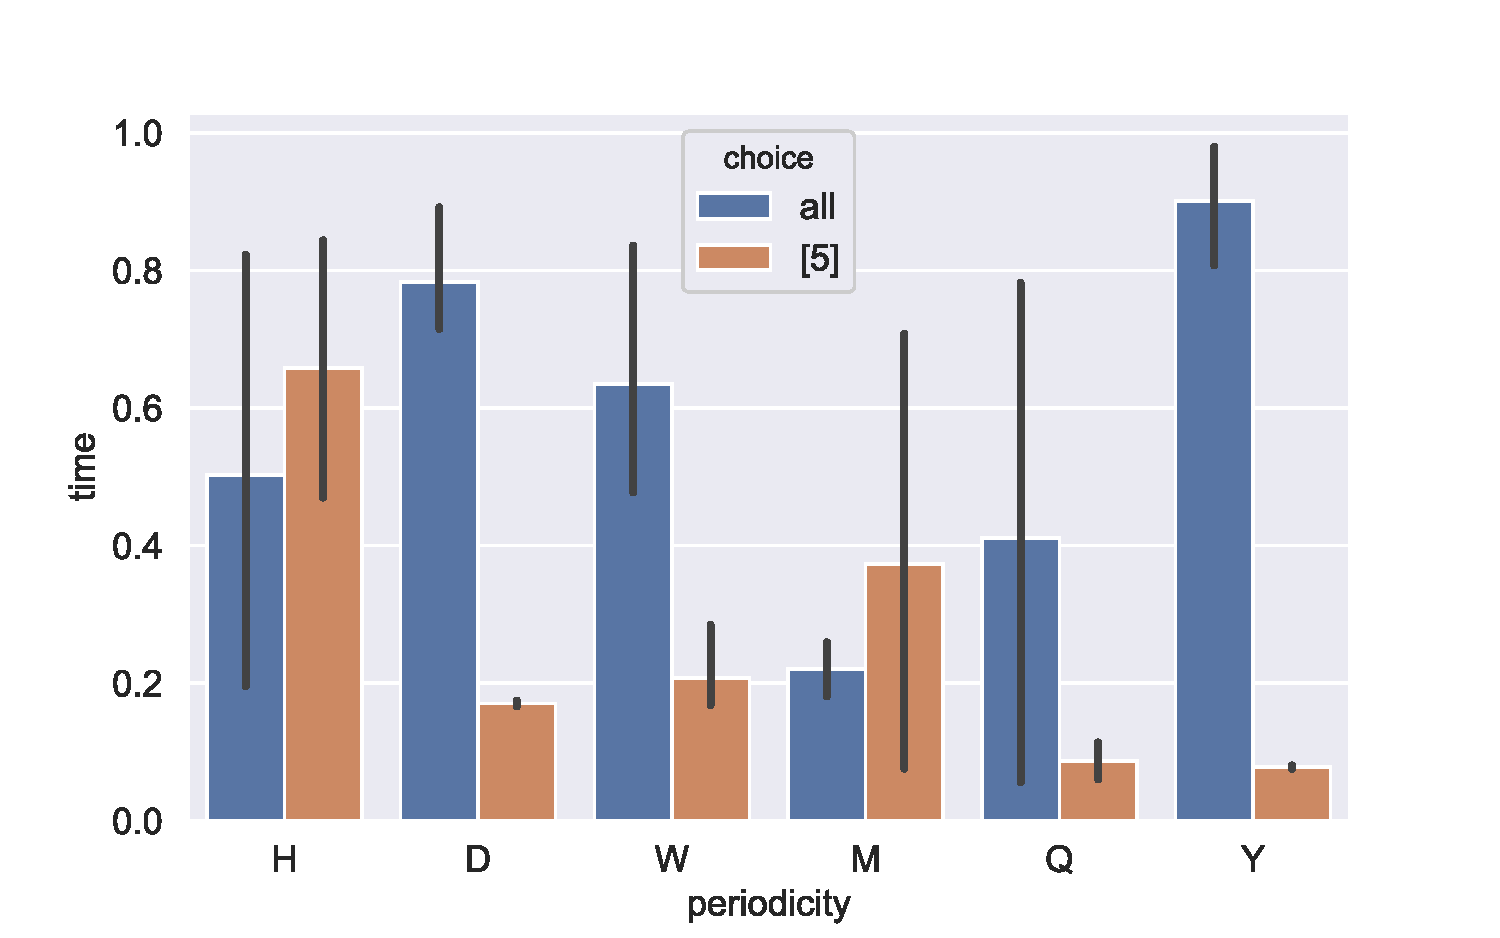
\includegraphics[width=\linewidth]{pictures/hyper-learning_steps-time.pdf}
				\caption{Время до сходимости \\ против выбора обучающих шагов}
				\label{hyper:learning_steps:time}
			\end{subfigure}%
			\begin{subfigure}[b]{.5\linewidth}
				\centering
				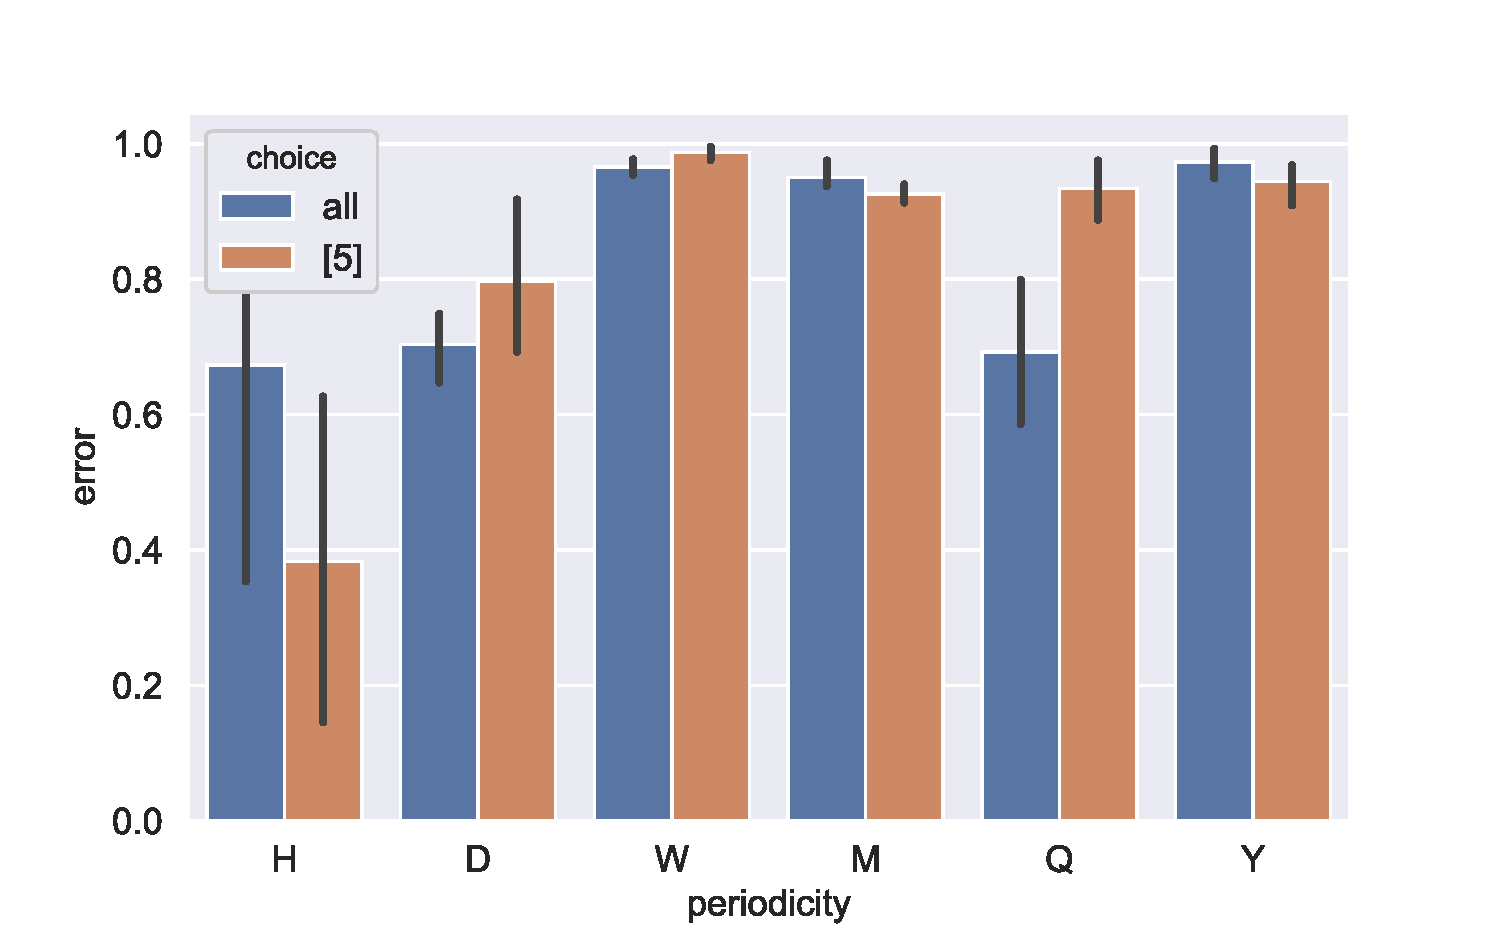
\includegraphics[width=\linewidth]{pictures/hyper-learning_steps-mse.pdf}
				\subcaption{MSE на тестирующей выборке \\ против выбора обучающих шагов}
				\label{hyper:learning_steps:mse}
			\end{subfigure}
			\caption{Сравнение моделей с различным выбором обучающих шагов}
			\label{hyper:learning_steps}
		\end{figure}
		\newpage
  		\item[2)] Значение гиперпараметра \texttt{ar\_depth} подбиралось по сетке [1, 5, 10, 15, 20, 25, 30]. Как видно на графиках \ref{hyper:ar_depth}, на половине выбранных рядов лучший MSE случается при \texttt{ar\_depth} $ = 1$, поэтому именно это значение было зафиксировано. Тем не менее, в случае \texttt{ar\_depth} нужно понимать, что этот гиперпараметр нужно подбирать отдельно для каждого временного ряда.
		\begin{figure}[!h]
			\captionsetup{justification=centering}
			\begin{subfigure}[b]{.5\linewidth}
				\centering
				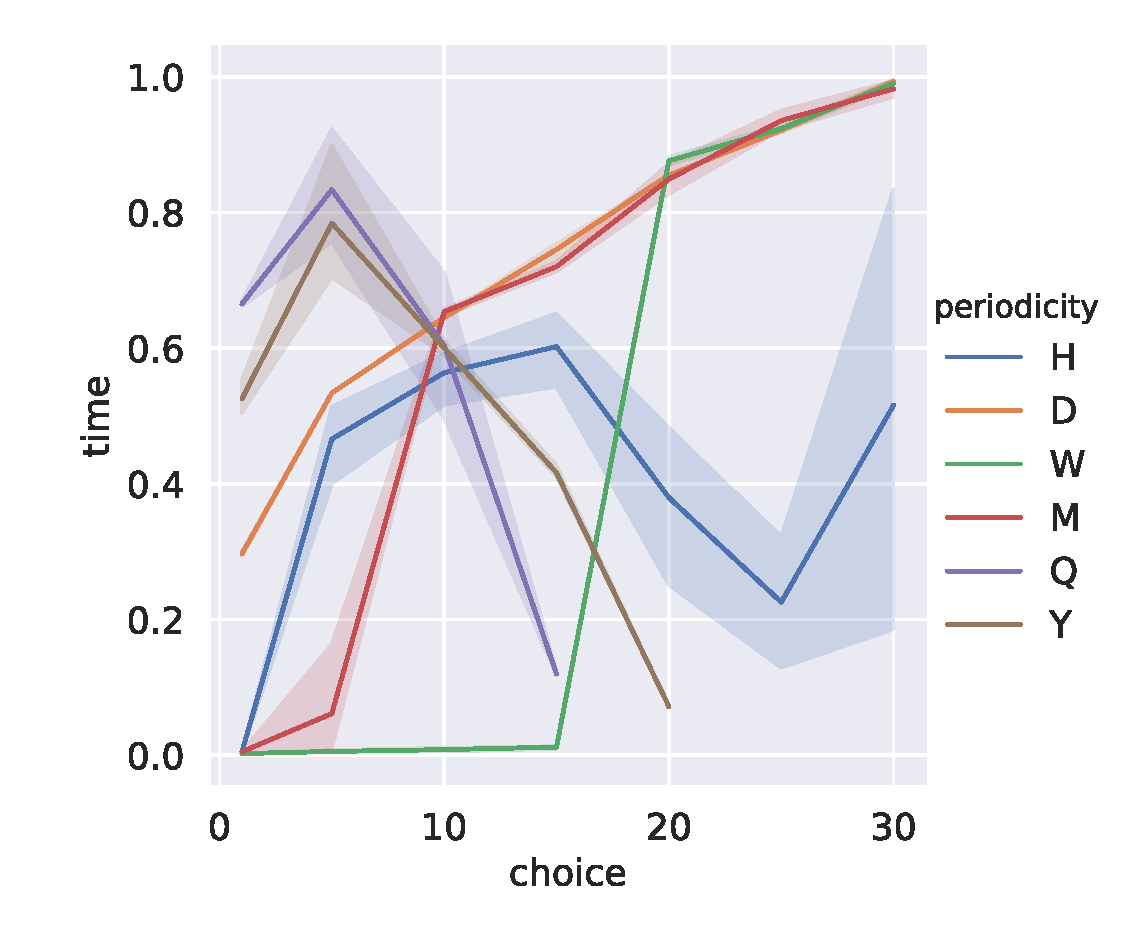
\includegraphics[width=\linewidth]{pictures/hyper-ar_depth-time.pdf}
				\caption{Время до сходимости \\ против глубины авторегрессии}
				\label{hyper:ar_depth:time}
			\end{subfigure}%
			\begin{subfigure}[b]{.5\linewidth}
				\centering
				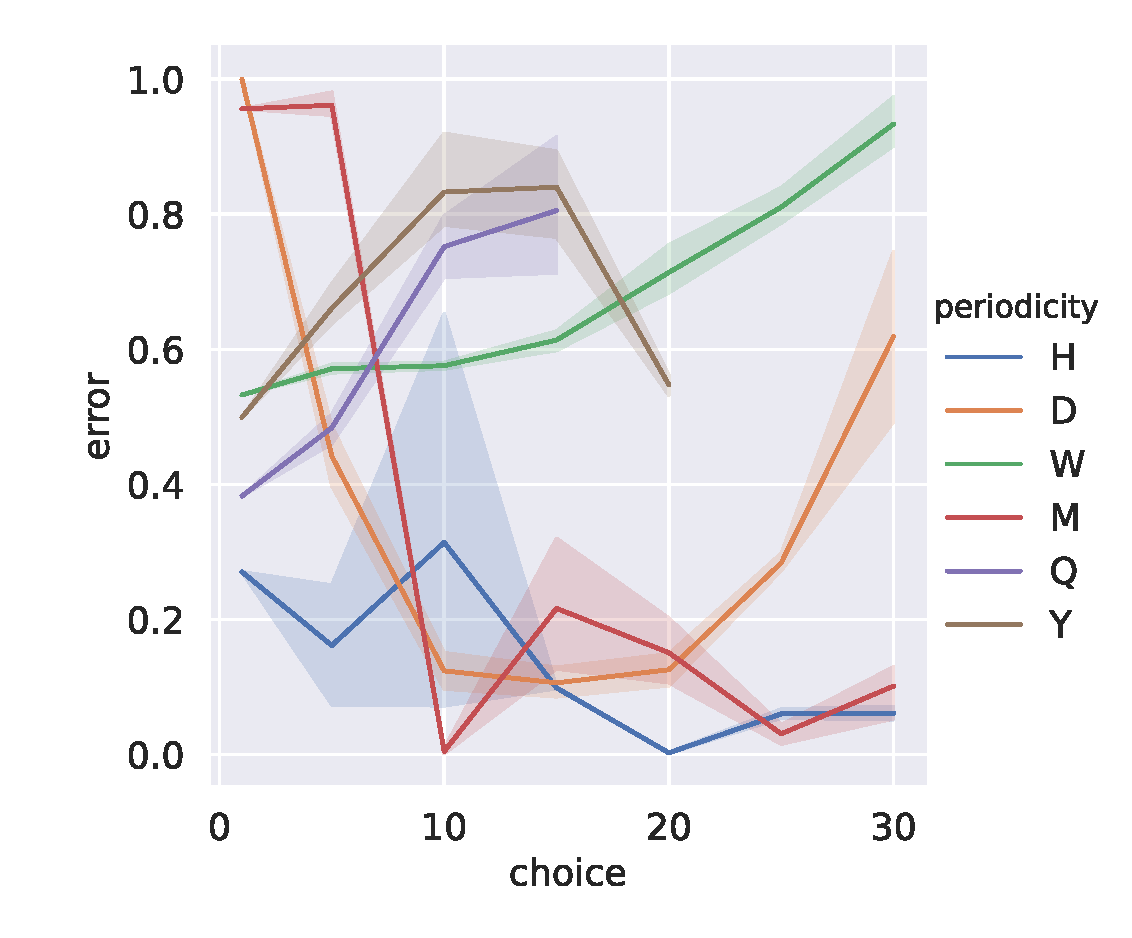
\includegraphics[width=\linewidth]{pictures/hyper-ar_depth-mse.pdf}
				\subcaption{MSE на тестирующей выборке \\ против глубины авторегрессии}
				\label{hyper:ar_depth:mse}
			\end{subfigure}
			\caption{Сравнение моделей с различной глубиной авторегрессии}
			\label{hyper:ar_depth}
		\end{figure}
    	\item[3)] Для тестирования гиперпараметра \texttt{seas\_depth} отдельно для каждой периодичности, кроме годовой (годовые данные в этом тестировании не участвовали в силу того, что они обычно не сезонны) были выбраны некоторые стандартные периоды сезонности -- для часовых данных 24, для дневных 30, для недельных 4 (месяц), для месячных 12, для квартальных 4. После этого гиперпараметр \texttt{seas\_depth} перебирался по сетке [1, 2, 3, 4]. Как результат получаем (с графиков \ref{hyper:seas_depth}), что лучший \texttt{seas\_depth} $ = 1$.
		\begin{figure}[!h]
			\captionsetup{justification=centering}
			\begin{subfigure}[b]{.5\linewidth}
				\centering
				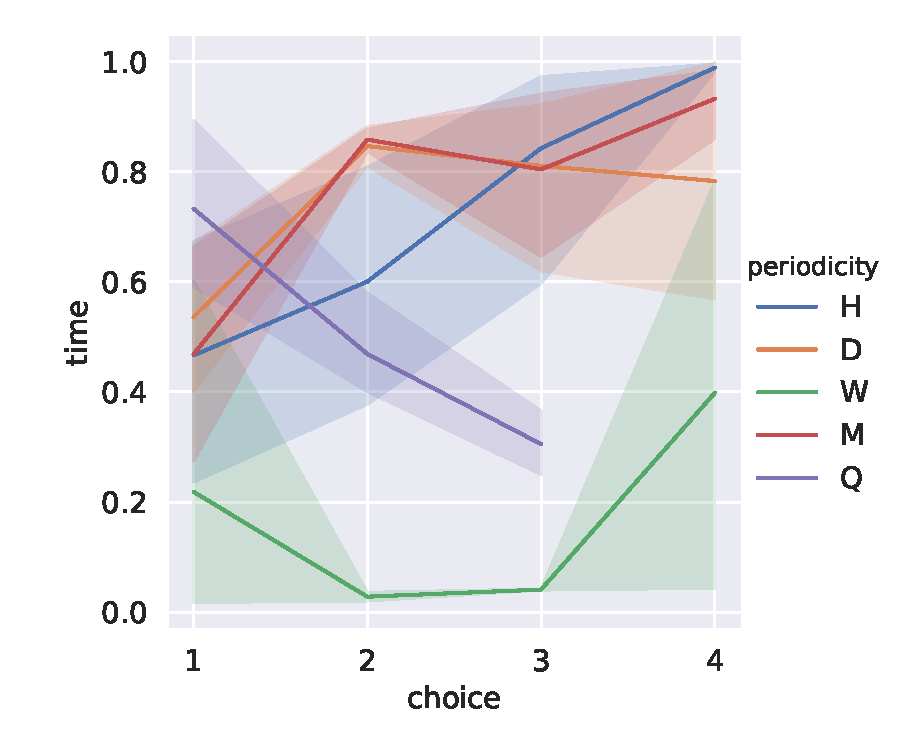
\includegraphics[width=\linewidth]{pictures/hyper-seas_depth-time.pdf}
				\caption{Время до сходимости \\ против глубины сезонной авторегрессии}
				\label{hyper:seas_depth:time}
			\end{subfigure}%
			\begin{subfigure}[b]{.5\linewidth}
				\centering
				
\includegraphics[width=\linewidth]{pictures/hyper-seas_depth-mse.pdf}
				\subcaption{MSE на тестирующей выборке \\ против глубины сезонной авторегрессии}
				\label{hyper:seas_depth:mse}
			\end{subfigure}
			\caption{Сравнение моделей с различной глубиной сезонной авторегрессии}
			\label{hyper:seas_depth}
		\end{figure}		
     	\item[4)] Понятно, что гиперпараметр \texttt{fit\_intercept} выбирался среди значений [\texttt{True}, \texttt{False}]. По графикам \ref{hyper:fit_intercept} видно, что модели почти не отличаются по MSE, но прим этом немного быстрее обучается модель, в которой отступ обучается, поэтому решили обучать отступ.
		\begin{figure}[!h]
			\captionsetup{justification=centering}
			\begin{subfigure}[b]{.5\linewidth}
				\centering
				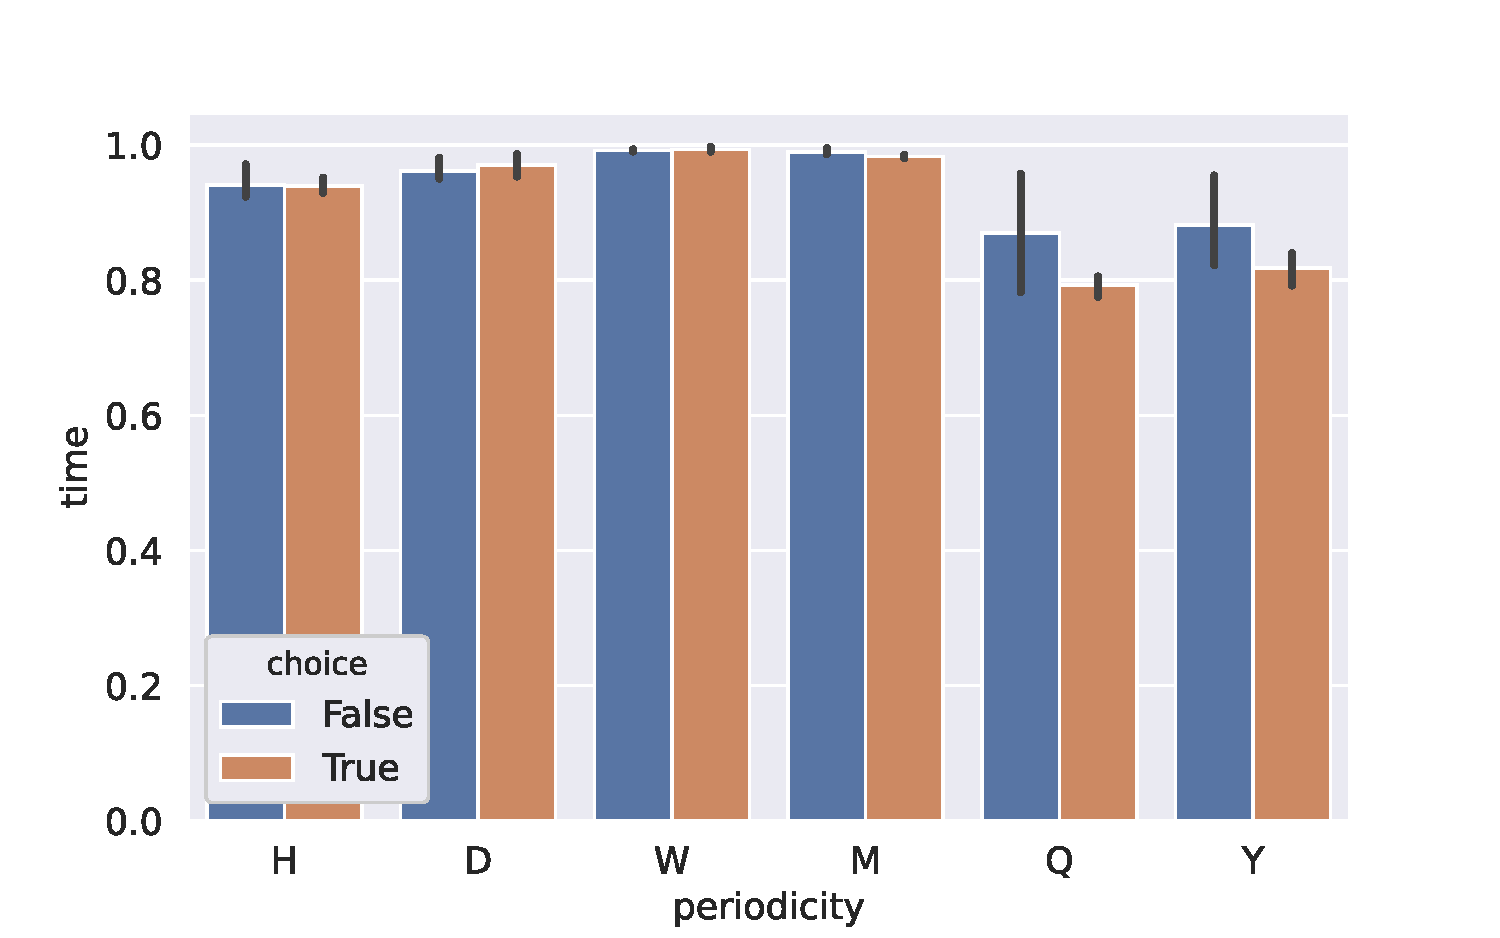
\includegraphics[width=\linewidth]{pictures/hyper-fit_intercept-time.pdf}
				\caption{Время до сходимости \\ против выбора обучения отступа}
				\label{hyper:fit_intercept:time}
			\end{subfigure}%
			\begin{subfigure}[b]{.5\linewidth}
				\centering
				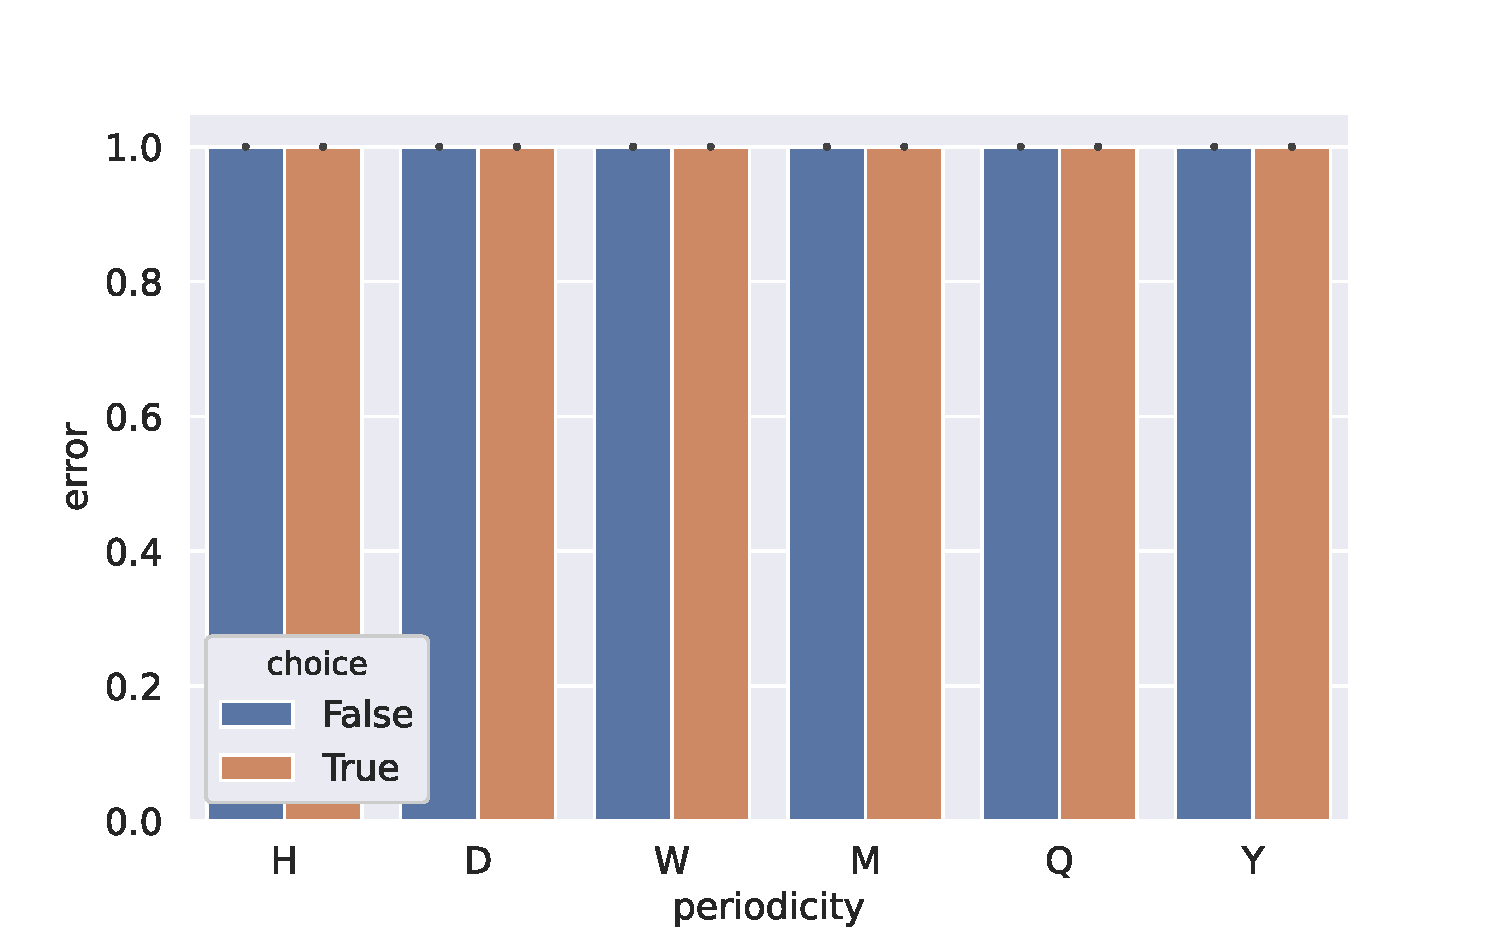
\includegraphics[width=\linewidth]{pictures/hyper-fit_intercept-mse.pdf}
				\subcaption{MSE на тестирующей выборке \\ против выбора обучения отступа}
				\label{hyper:fit_intercept:mse}
			\end{subfigure}
			\caption{Сравнение моделей с обученным отступом и без}
			\label{hyper:fit_intercept}
		\end{figure}
		
      	\item[5)] Параметр \texttt{tolerance} подбирался по логарифмической сетке от 1 до $10^{-8}$. По графикам \ref{hyper:tolerance} видно, что MSE на тестирующей выборке для 66\% рядов выросло, когда мы хоть немного начали обучать модель, и из-за этого лучшим выбором, возможно, был бы \texttt{tolerance} $ = 1$. Однако это бы значило, что мы совсем ничего не обучаем, поэтому было решено взять \texttt{tolerance} всё-таки поменьше. Видно, что также на 66\% рядов качество на тестирующей выборке немного растёт при \texttt{tolerance} $ = 10^{-2}$, поэтому было решено взять именно такую точность. 
		\begin{figure}[!h]
			\captionsetup{justification=centering}
			\begin{subfigure}[b]{.5\linewidth}
				\centering
				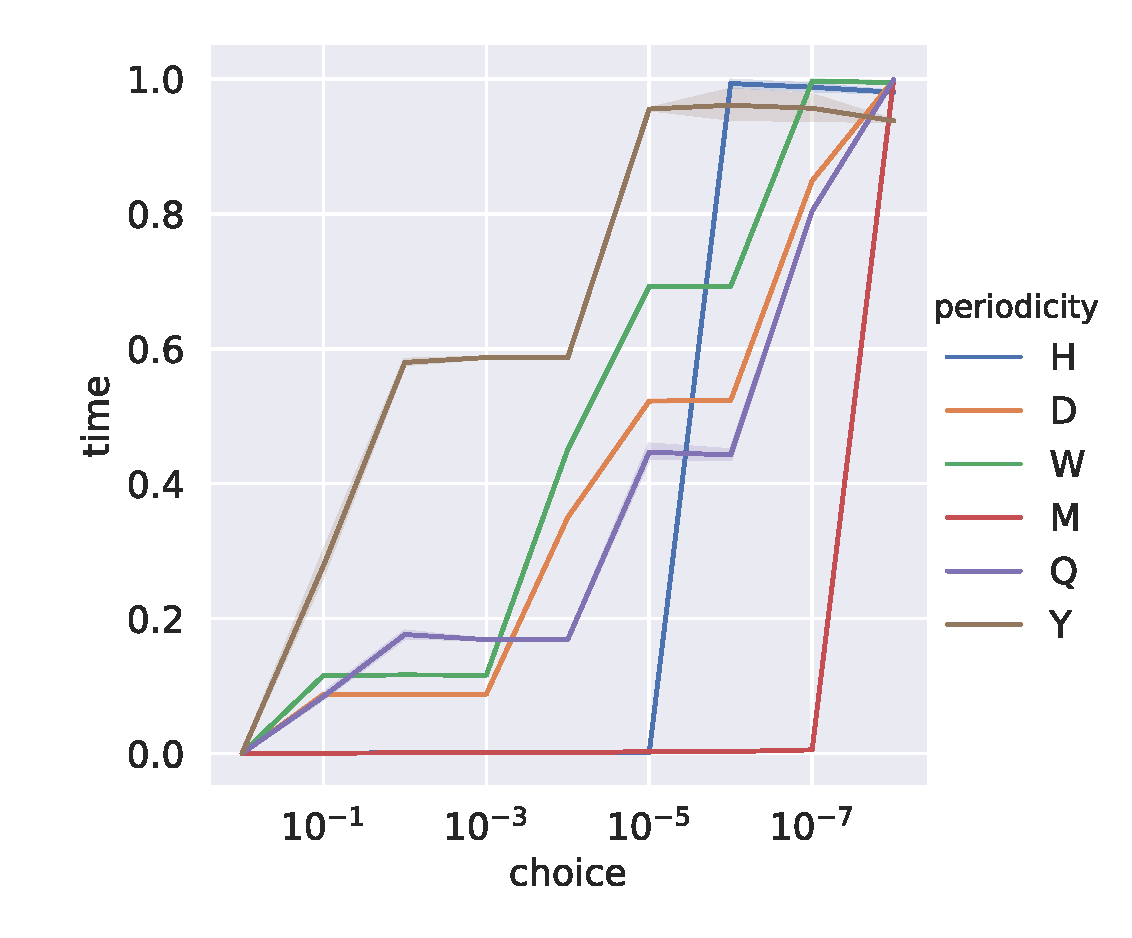
\includegraphics[width=\linewidth]{pictures/hyper-tolerance-time.pdf}
				\caption{Время до сходимости \\ против выбора точности}
				\label{hyper:tolerance:time}
			\end{subfigure}%
			\begin{subfigure}[b]{.5\linewidth}
				\centering
				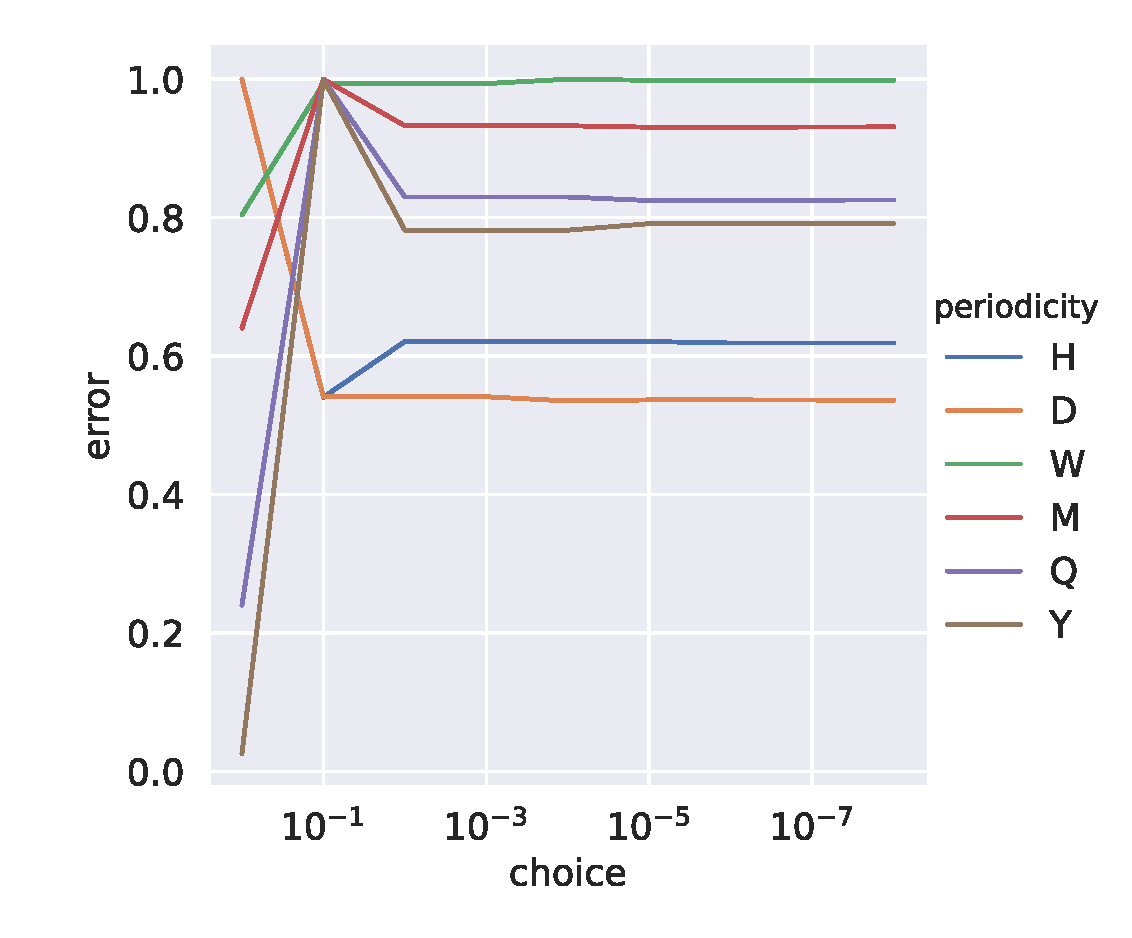
\includegraphics[width=\linewidth]{pictures/hyper-tolerance-mse.pdf}
				\subcaption{MSE на тестирующей выборке \\ против выбора точности}
				\label{hyper:tolerance:mse}
			\end{subfigure}
			\caption{Сравнение моделей, обученных с разной точностью}
			\label{hyper:tolerance}
		\end{figure}
       	\item[6)] Задача параметра \texttt{max\_iter} --- быть достаточно большим, чтобы большинство рядов сходилось к заданной точности, но не быть слишком большим, чтобы модель не зависала на \textquotedblleft плохих\textquotedblright\ рядах. В ходе эксперимента было выяснено, что все 6 рядов сходятся к заданной точности за 10 итераций, таким образом, это значение было выбрано как значение по умолчанию.
        \item[7)] Мы разобрались с гиперпараметрами самой модели, теперь надо разобраться с параметрами обучения. Первый гиперпараметр --- это метод выбора стартового вектора параметров. Опции для этого гиперпараметра такие:
		\begin{itemize}
			\item Выбирать стартовые параметры случайно (и отнормировать, чтобы сумма была равна 1);
   			\item Сделать их равными частным автокорреляциям значений ряда с соответствующими лагами;
      		\item Cделать равным частным автокорреляциям и отнормировать.
		\end{itemize}
		Так как бесполезно сравнивать эти методы с \texttt{ar\_depth} $ = 1$ (нормирование приводит к тому, что первый и третий методы совпадают), хотя это и сделано на графиках \ref{hyper:starting_params_1}, я попробовал сравнить их с \texttt{ar\_depth} $ = 15$ на графиках \ref{hyper:starting_params_15}. Получилось, что с точки зрения качества выгоднее всего выбирать стартовый набор параметров случайно.
        \begin{figure}[!h]
			\captionsetup{justification=centering}
			\begin{subfigure}[b]{.5\linewidth}
				\centering
				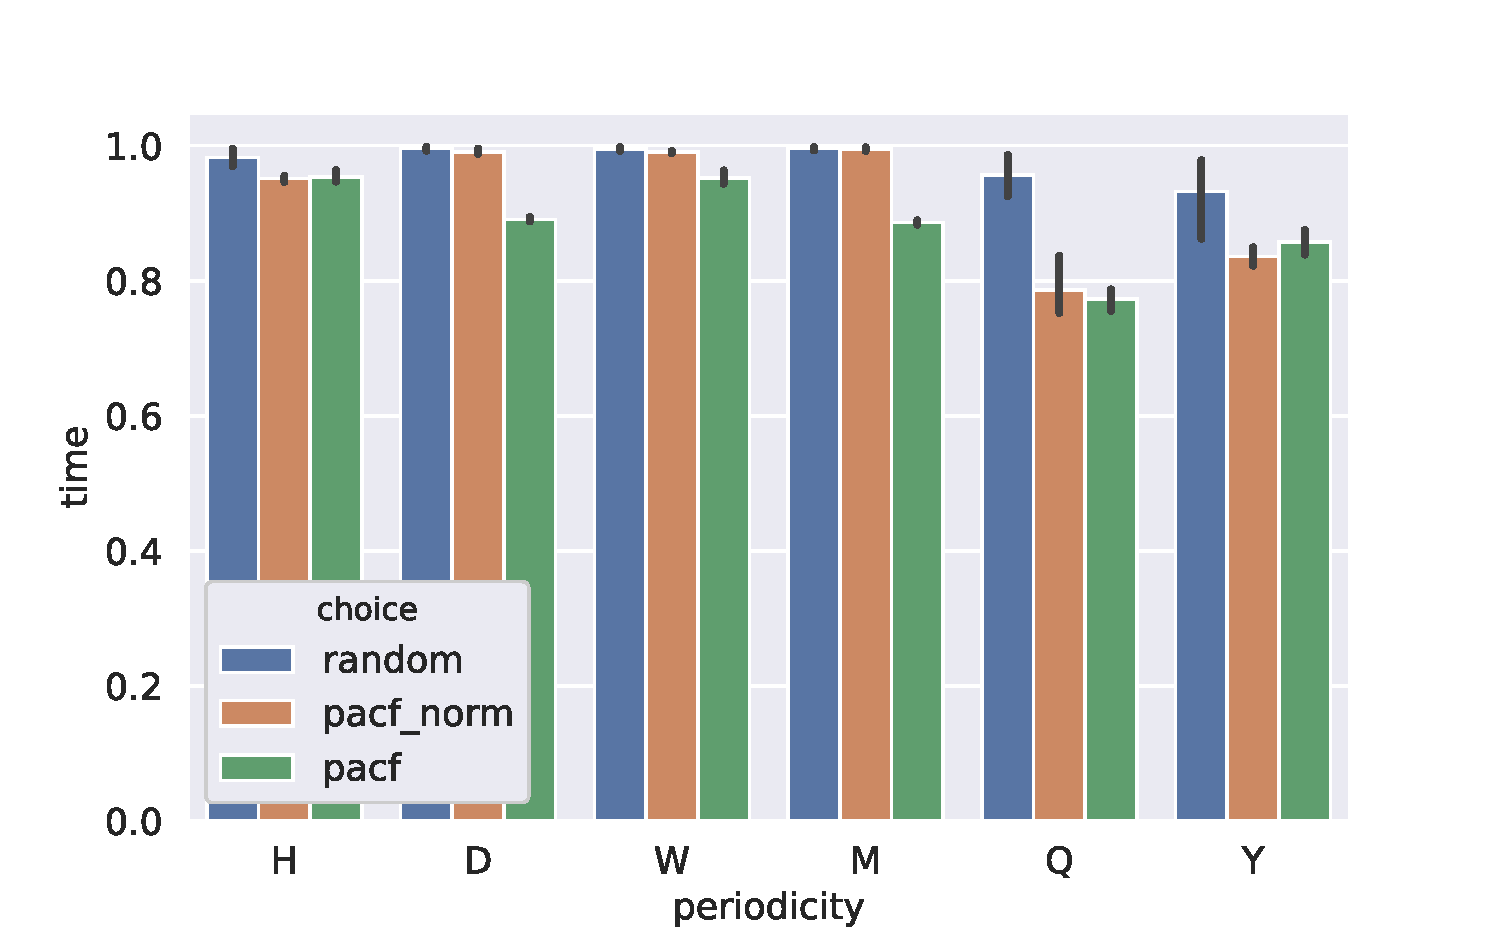
\includegraphics[width=\linewidth]{pictures/hyper-starting_params-time.pdf}
				\caption{Время до сходимости \\ против метода выбора стартовых параметров}
				\label{hyper:starting_params_1:time}
			\end{subfigure}%
			\begin{subfigure}[b]{.5\linewidth}
				\centering
				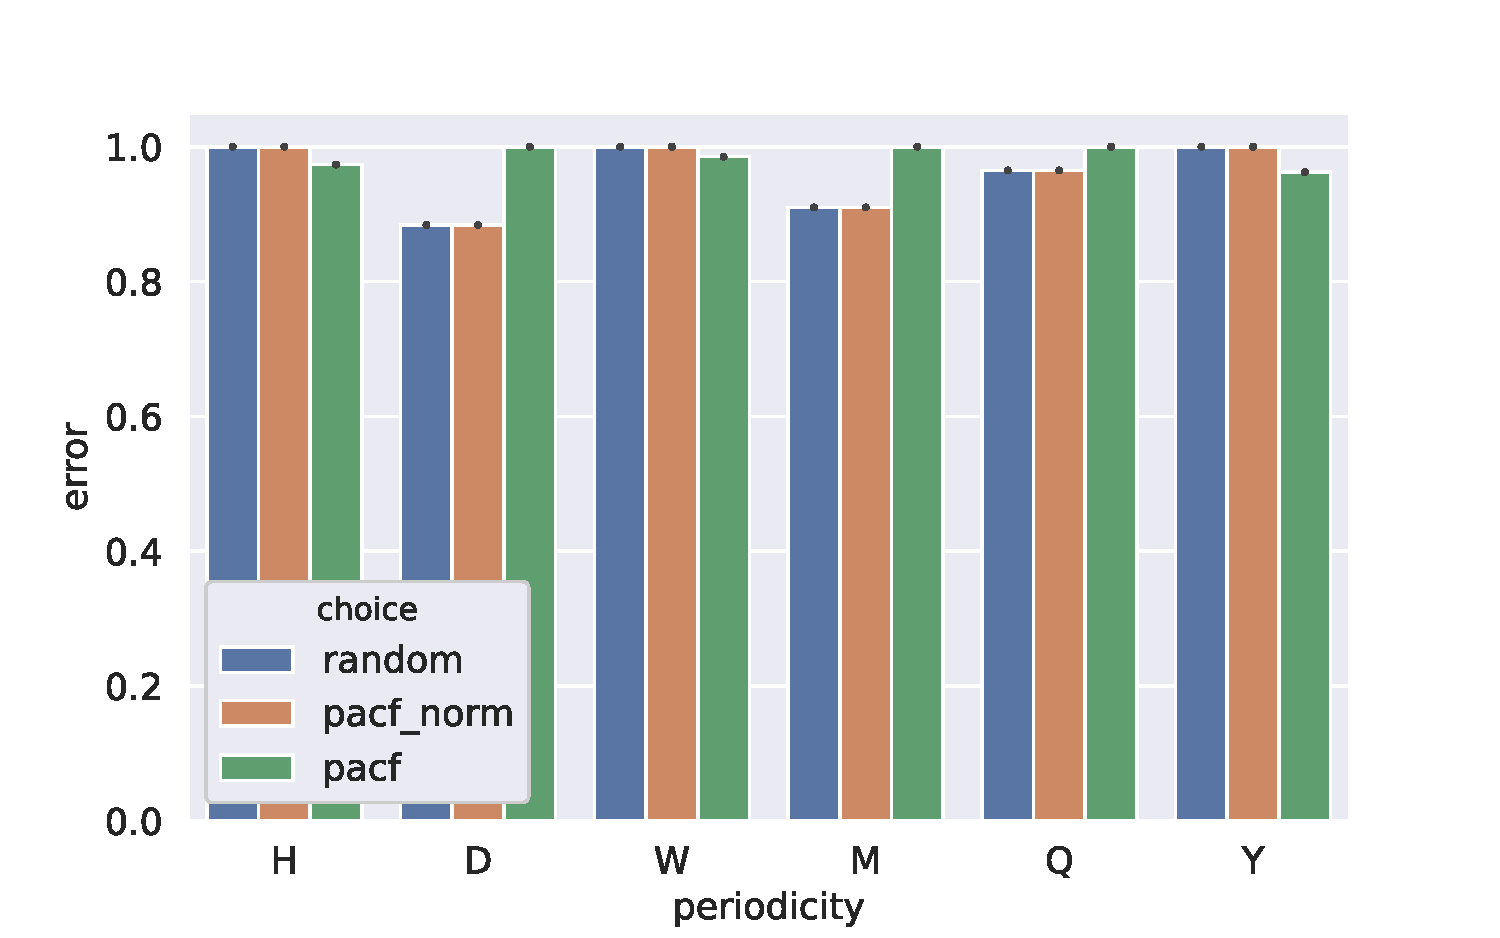
\includegraphics[width=\linewidth]{pictures/hyper-starting_params-mse.pdf}
				\subcaption{MSE на тестирующей выборке \\ против метода выбора стартовых параметров}
				\label{hyper:starting_params_1:mse}
			\end{subfigure}
			\caption{Сравнение моделей с различным методом \\ выбора стартовых параметров \\ (\texttt{ar\_depth = 1})}
			\label{hyper:starting_params_1}
		\end{figure}
		\begin{figure}[!h]
			\captionsetup{justification=centering}
			\begin{subfigure}[b]{.5\linewidth}
				\centering
				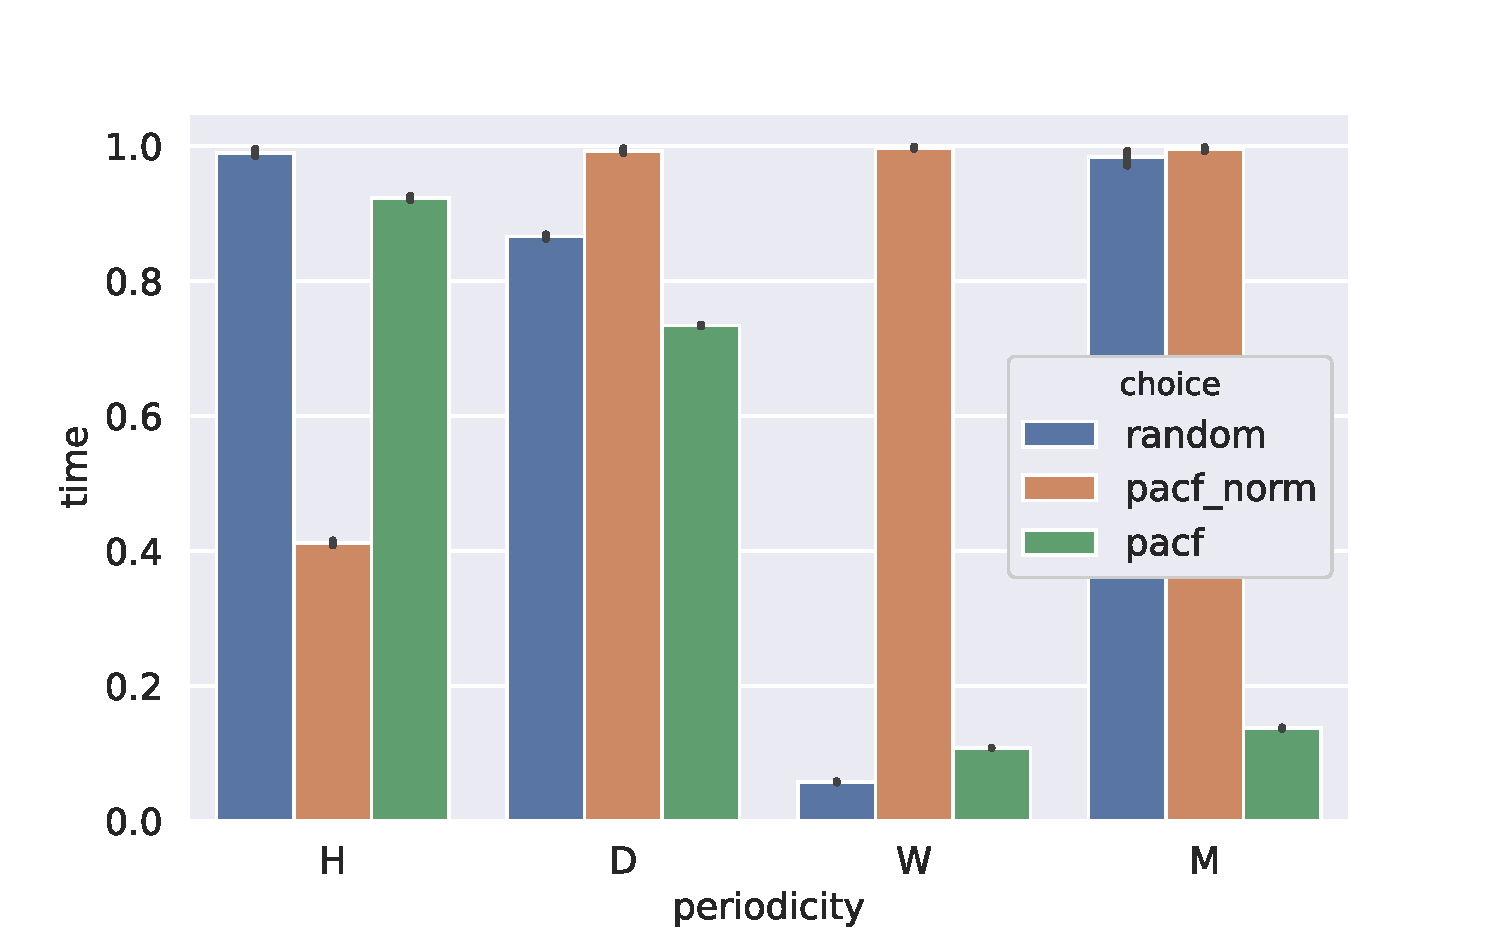
\includegraphics[width=\linewidth]{pictures/hyper-starting_params_normalized-time.pdf}
				\caption{Время до сходимости \\ против метода выбора стартовых параметров}
				\label{hyper:starting_params_15:time}
			\end{subfigure}%
			\begin{subfigure}[b]{.5\linewidth}
				\centering
				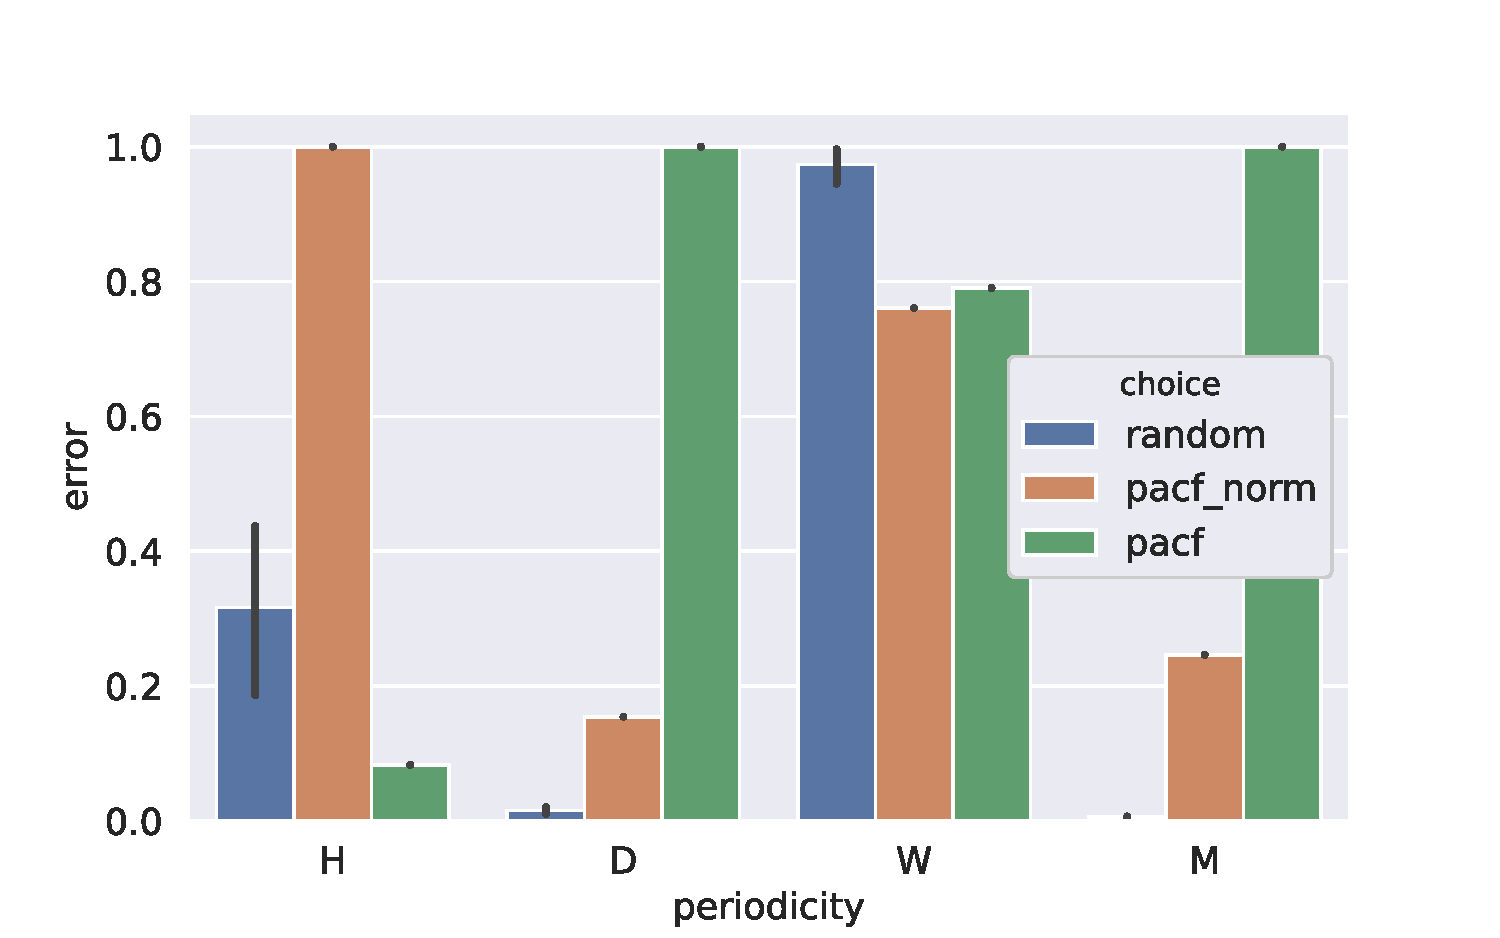
\includegraphics[width=\linewidth]{pictures/hyper-starting_params_normalized-mse.pdf}
				\subcaption{MSE на тестирующей выборке \\ против метода выбора стартовых параметров}
				\label{hyper:starting_params_15:mse}
			\end{subfigure}
			\caption{Сравнение моделей с различным методом \\ выбора стартовых параметров \\ (\texttt{ar\_depth = 15})}
			\label{hyper:starting_params_15}
		\end{figure}
        \item[8)] Также были отобраны метод выбора длины шага как гиперпараметр по умолчанию. Этот гиперпараметр, в теории, никак не должен влиять на качество модели, а только на время сходимости, поэтому я построил график времени сходимости против выбора длины шага: \ref{hyper:lr_finder}. Оказалось, что для динамических моделей быстрее всего выбирать длину шага по формуле $\alpha_k = \lambda \cdot \left( \frac{s_0}{s_0 + k} \right)^p$, где $\lambda = 5 \cdot 10^{-3},\,s_0 = 1,\, p = 0.5$.
        \begin{figure}[!h]
			\captionsetup{justification=centering}
			\centering
			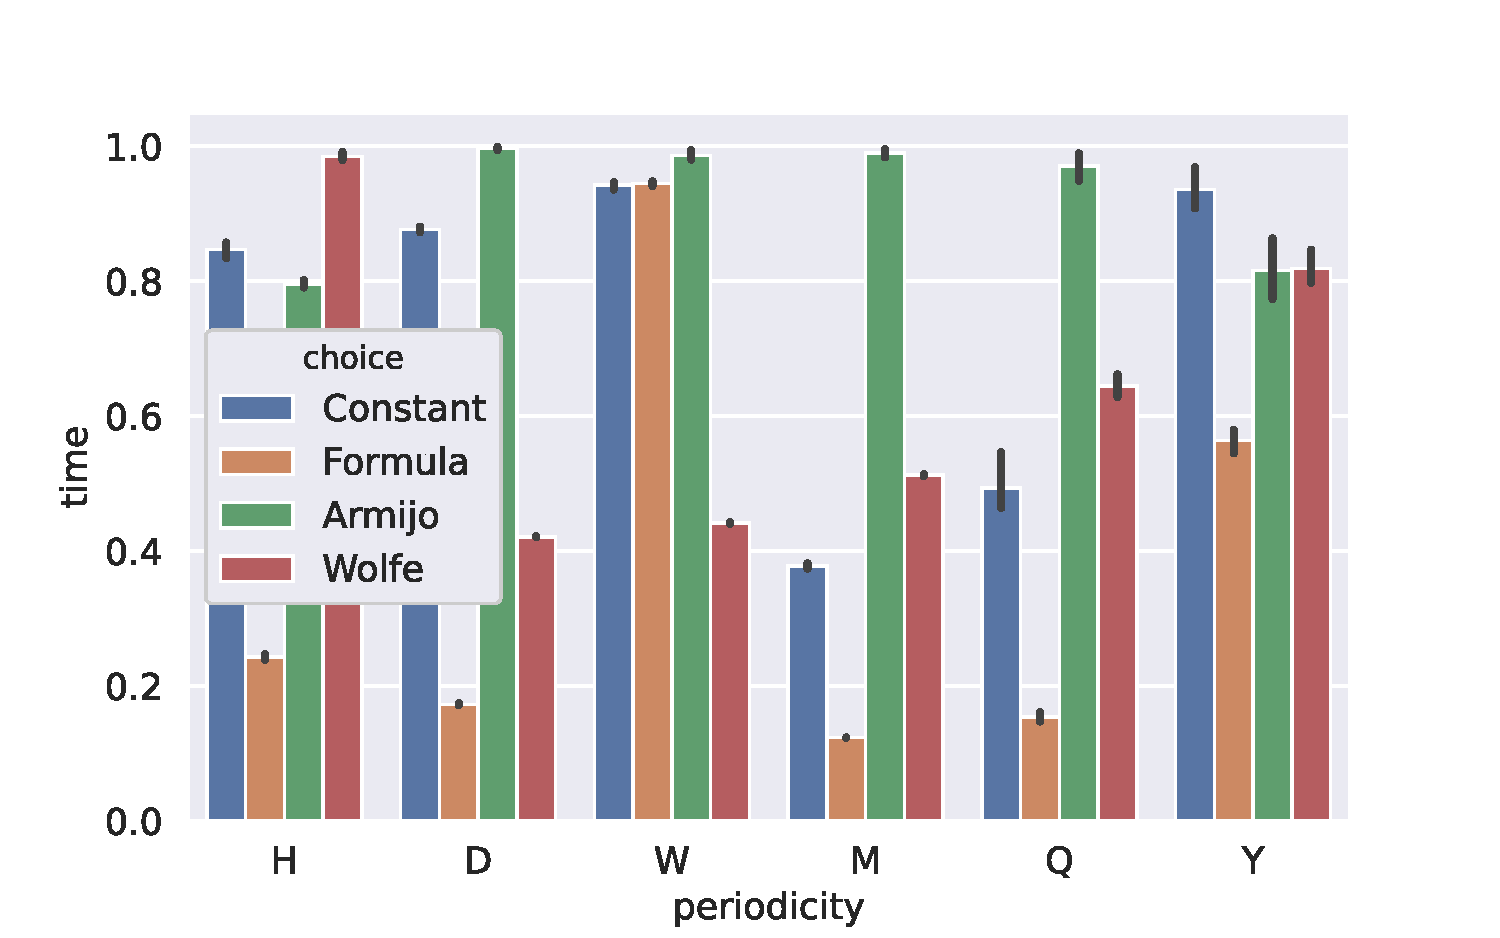
\includegraphics[width=\linewidth]{pictures/hyper-lr_finder-time.pdf}
			\caption{Время до сходимости моделей с различным методом выбора длины шага}
			\label{hyper:lr_finder}
		\end{figure}
	\end{enumerate}
\section{Описание поставленного эксперимента}
	\subsection{Данные}
	Для сравнения динамических моделей с базовыми методами были использованы временные ряды из выборки M4. Данная выборка содержит 100000 рядов разной периодичности и из разных источников. В деталях можно отобразить разбиение рядов по категориям с помощью таблицы: \ref{exp:m4}.
	\begin{table}[!h]
		\captionsetup{justification=centering}
		\centering
		\caption{Категоризация рядов в выборке M4}
		\begin{tabular}{llllllll}
			\hline 
			 & Demographic & Finance & Industry & Macro & Micro & Other & Total\\
			\hline 
			Yearly & 1088 & 6519 & 3716 & 3903 & 6538 & 1236 & 23000\\
			Quarterly & 1858 & 5305 & 4637 & 5315 & 6020 & 865 & 24000\\
			Monthly & 5728 & 10987 & 10017 & 10016 & 10975 & 277 & 48000\\
			Weekly & 24 & 164 & 6 & 41 & 112 & 12 & 359\\
			Daily & 10 & 1559 & 422 & 127 & 1476 & 633 & 4227\\
			Hourly & 0 & 0 & 0 & 0 & 0 & 414 & 414\\
			Total & 8708 & 24354 & 18798 & 19402 & 25121 & 3437 & 100000\\
			\hline
		\end{tabular}
		\label{exp:m4}
	\end{table}

	Данные предобрабатывались следующим образом. Мы хотели получить разбиение рядов по нескольким признакам, а именно периодичности, источнику, наличию сезонности (считалось, что ряд сезонный, если сила сезонности в алгоритме разложения STL (\bibref{cleveland90}{Cleveland R. B. et al.}{1990}) больше или равна 0.2) и стационарности ряда по тренду image.pdf(стационарность тестировалась с помощью теста KPSS (\bibref{kwiatkowski92}{Kwiatkowski D.et al.}{1992})). При этом для каждого \textquotedblleft кластера\textquotedblright\ нам нужно было провести статистические тесты о доле, чтобы сравнить нашу модель с какой-то другой. Для этого нам нужно было, чтобы в каждом кластере было достаточно много рядов, например, от 200. Но при этом мы не хотели тратить слишком много времени на вычисления, поэтому все кластеры, которые содержали больше 200 рядов, обрезались до 200 рядов. Итоговую выборку и разбиение на кластеры можно описать этой таблицей: \ref{exp:m4_clusterized}. В ней бинарные значения в ячейках означают, был ли данный кластер взят в выборку. Столбцы y/n означают, являются ли ряды в соответствующем кластере стационарными; строки y/n -- являются ли они сезонными. Например, единица в строке Yearly/y и столбце Demographic/n означает, что в анализ был включён кластер сезонных нестационарных рядов с годовой перодичностью из демографических данных.
	\begin{table}[!h]
		\captionsetup{justification=centering}
		\centering
		\caption{Расширенная категоризация рядов в выборке M4}
		\begin{tabular}{ccccccccccccccc}
			\hline 
			\multicolumn{2}{c}{} & \multicolumn{2}{c}{Demographic} & \multicolumn{2}{c}{Finance} & \multicolumn{2}{c}{Industry} & \multicolumn{2}{c}{Macro} & \multicolumn{2}{c}{Micro} & \multicolumn{2}{c}{Other} & Total\\ 
			\hline 
			\multicolumn{2}{c}{} 			& y & n & y & n & y & n & y & n & y & n & y & n &  \\
			\multirow{2}{*}{Yearly} 	& y & 0 & 1 & 1 & 1 & 1 & 1 & 1 & 1 & 1 & 1 & 1 & 1 & 11\\
										 & n & 0 & 1 & 0 & 1 & 0 & 1 & 0 & 1 & 0 & 1 & 0 & 0 & 5\\
			\multirow{2}{*}{Quarterly} 	& y & 1 & 1 & 1 & 1 & 1 & 1 & 1 & 1 & 1 & 1 & 0 & 1 & 11\\
										 & n & 0 & 1 & 0 & 1 & 1 & 1 & 1 & 1 & 1 & 1 & 0 & 0 & 8\\
			\multirow{2}{*}{Monthly} 	& y & 1 & 1 & 1 & 1 & 1 & 1 & 1 & 1 & 1 & 1 & 0 & 0 & 10\\
										 & n & 0 & 1 & 1 & 1 & 1 & 1 & 1 & 1 & 1 & 1 & 0 & 0 & 9\\
			\multirow{2}{*}{Weekly} 	& y & 0 & 0 & 0 & 0 & 0 & 0 & 0 & 0 & 0 & 0 & 0 & 0 & 0\\
										 & n & 0 & 0 & 0 & 0 & 0 & 0 & 0 & 0 & 0 & 0 & 0 & 0 & 0\\
			\multirow{2}{*}{Daily}  	& y & 0 & 0 & 0 & 1 & 0 & 1 & 0 & 0 & 0 & 1 & 0 & 1 & 4\\
										 & n & 0 & 0 & 0 & 0 & 0 & 0 & 0 & 0 & 0 & 0 & 0 & 0 & 0\\
			\multirow{2}{*}{Hourly} 	& y & 0 & 0 & 0 & 0 & 0 & 0 & 0 & 0 & 0 & 0 & 0 & 0 & 0\\
										 & n & 0 & 0 & 0 & 0 & 0 & 0 & 0 & 0 & 0 & 0 & 0 & 1 & 1\\
			Total 				 		&   & 2 & 6 & 4 & 7 & 5 & 7 & 5 & 6 & 5 & 7 & 1 & 4 & 59\\
			\hline
		\end{tabular}
		\label{exp:m4_clusterized}
	\end{table}
	\subsection{Постановка эксперимента}
	Данный эксперимент ставит перед собой две основные задачи:
	\begin{enumerate}
		\item[1)] Статистическое сравнение динамических моделей с базовыми методами как в целом, так и на отдельных кластерах рядов;
  		\item[2)] Выявление свойств рядов и горизонтов прогнозирования, на которых динамические регрессионные модели выдают лучшее качество относительно базовых методов.
	\end{enumerate}
	Чтобы выполнить эти задачи, для начала для каждого ряда из собранных кластеров и для каждого горизонта прогнозирования были запущены следующие модели:
	\begin{itemize}
		\item Базовые, то есть наивная, ETS, ARIMA, PROPHET;
  		\item Обычная динамическая регрессия, причём глубина авторегрессии перебиралась от 1 до 5, то есть всего таких моделей было запущено по пять на каждый ряд;
    	\item Сезонная динамическая регрессия, причём глубина авторегрессии перебиралась от 1 до 5, а глубина сезонной авторегрессии --- от 1 до 2, то есть всего таких моделей было запущено по десять на каждый ряд.
	\end{itemize} 
	При этом горизонты прогнозирования перебирались следующие:
	\begin{itemize}
		\item Одношаговый;
  		\item Многошаговый (при чём номер самого дальнего шага определялся периодичностью ряда --- так, для часовых данных это 24, для дневных --- 30, для месячных --- 12, для квартальных --- 4, а для годовых --- 10);
    	\item Прогноз на дальний шаг (последний среди соответствующего многошагового прогноза).
	\end{itemize}
	По вышеописанным правилам (как для горизонта прогнозирования) выбирался и период сезонности для сезонных динамических моделей; при этом для годовых данных сезонные динамические модели не запускались. После запуска моделей динамических регрессий для них брался минимум ошибки по разным параметрам. То есть, на выходе в столбцах таблицы должны быть базовые методы, а также динамическая регрессия и сезонная динамическая регрессия. Для базовых методов брались следующие реализации (все из библиотеки \texttt{sktime}): для ETS --- \texttt{sktime.forecasting.ets.AutoETS}, для ARIMA~--- \texttt{sktime.forecasting.arima.AutoARIMA}, для PROPHET --- \\\texttt{sktime.forecasting.fbprophet.Prophet}, для наивной модели --- \\\texttt{sktime.forecasting.naive.NaiveForecaster}. Дополнительно можно сказать о том, что если ряд оказывался слишком коротким, чтобы можно было эффективно обучиться, то он не рассматривается.

	Таким образом, после применения моделей и некоторых преобразований данных мы получим таблицу, в которой для каждого кластера и каждой модели
	лежит список ошибок модели на рядах из данного кластера. Мы считаем следующие статистики. Во-первых, для каждой модели мы считаем процент побед на рядах из данного кластера (то есть процент рядов, которые эта модель лучше всего предсказывает), а также по наибольшему числу побед выбираем лучшую модель на данном кластере. Во-вторых, для каждого базового метода мы проверяем гипотезу о доле, то есть гипотезу о том, что с вероятностью 0.5 динамическая модель показывает не худшее качество, чем рассматриваемый базовый метод, с уровнем значимости 0.95. Можно сказать, что таким образом мы проверяем гипотезу о том, что динамическая модель работает не хуже, чем рассматриваемый базовый метод. Опишем это более формально. Пусть доля побед динамической регрессии на рядах из кластера равна $P$. Тогда мы проверяем следimage.pngimage.pngimage.pngующие гипотезы:
	\begin{equation*}
		\begin{cases}
			H_0: P = 0.5 \\
			H_1: P < 0.5
		\end{cases}
	\end{equation*}
	В-третьих, на всех данных, кроме годовых, мы проверяем эти гипотезы и для сезонной динамической регрессии.

	\subsection{Проведение эксперимента}
	Вычисления в данном эксперименте запускались одновременно на двух машинах -- это Apple MacBook Pro (2021) с чипом Apple M1 Pro и оперативной памятью 32 GB на 9 потоках, а также на суперкомпьютере департамента прикладной экономики НИУ ВШЭ с оперативной памятью 251 GB на 47 потоках. Вычисления были выполнены в сумме примерно за 42 часа. Параллелльно здесь запускались именно процессы обучения моделей, это было выполнено с помощью библиотеки \texttt{multiprocessing}.

\section{Анализ полученных результатов}
	\subsection{Сравнение моделей}
	В данном разделе мы будем строить столбчатые диаграммы, на которых столбцами будут доли неотвергнутых гипотез о доле среди подмножества кластеров, объединённых по какому-то из признаков. Для начала нарисуем такие графики на всех кластерах для динамической и сезонной динамической регрессий: \ref{results:dynreg:full}, \ref{results:seasdynreg:full}. 
	\begin{figure}[!h]
		\captionsetup{justification=centering}
		\centering
		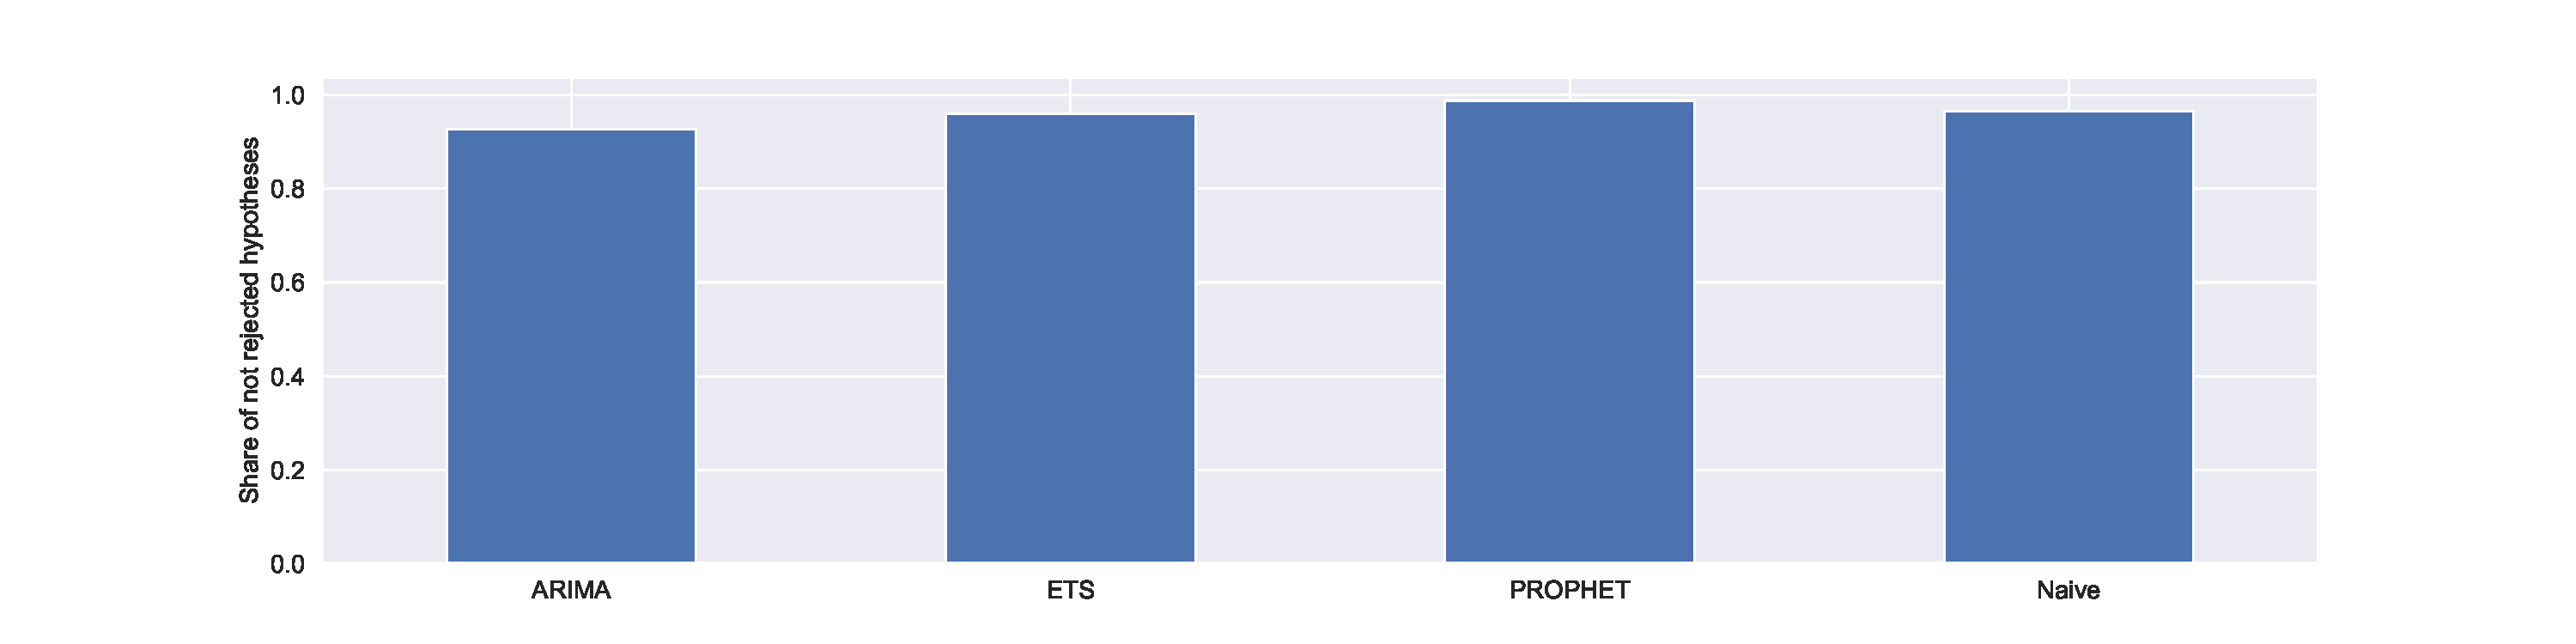
\includegraphics[width=\linewidth]{pictures/results-dynreg-full.pdf}
		\caption{Доли неотвергнутых гипотез о том, что динамическая регрессия \\ не хуже рассматриваемого базового метода}
		\label{results:dynreg:full}
	\end{figure}
	\begin{figure}[!h]
		\captionsetup{justification=centering}
		\centering
		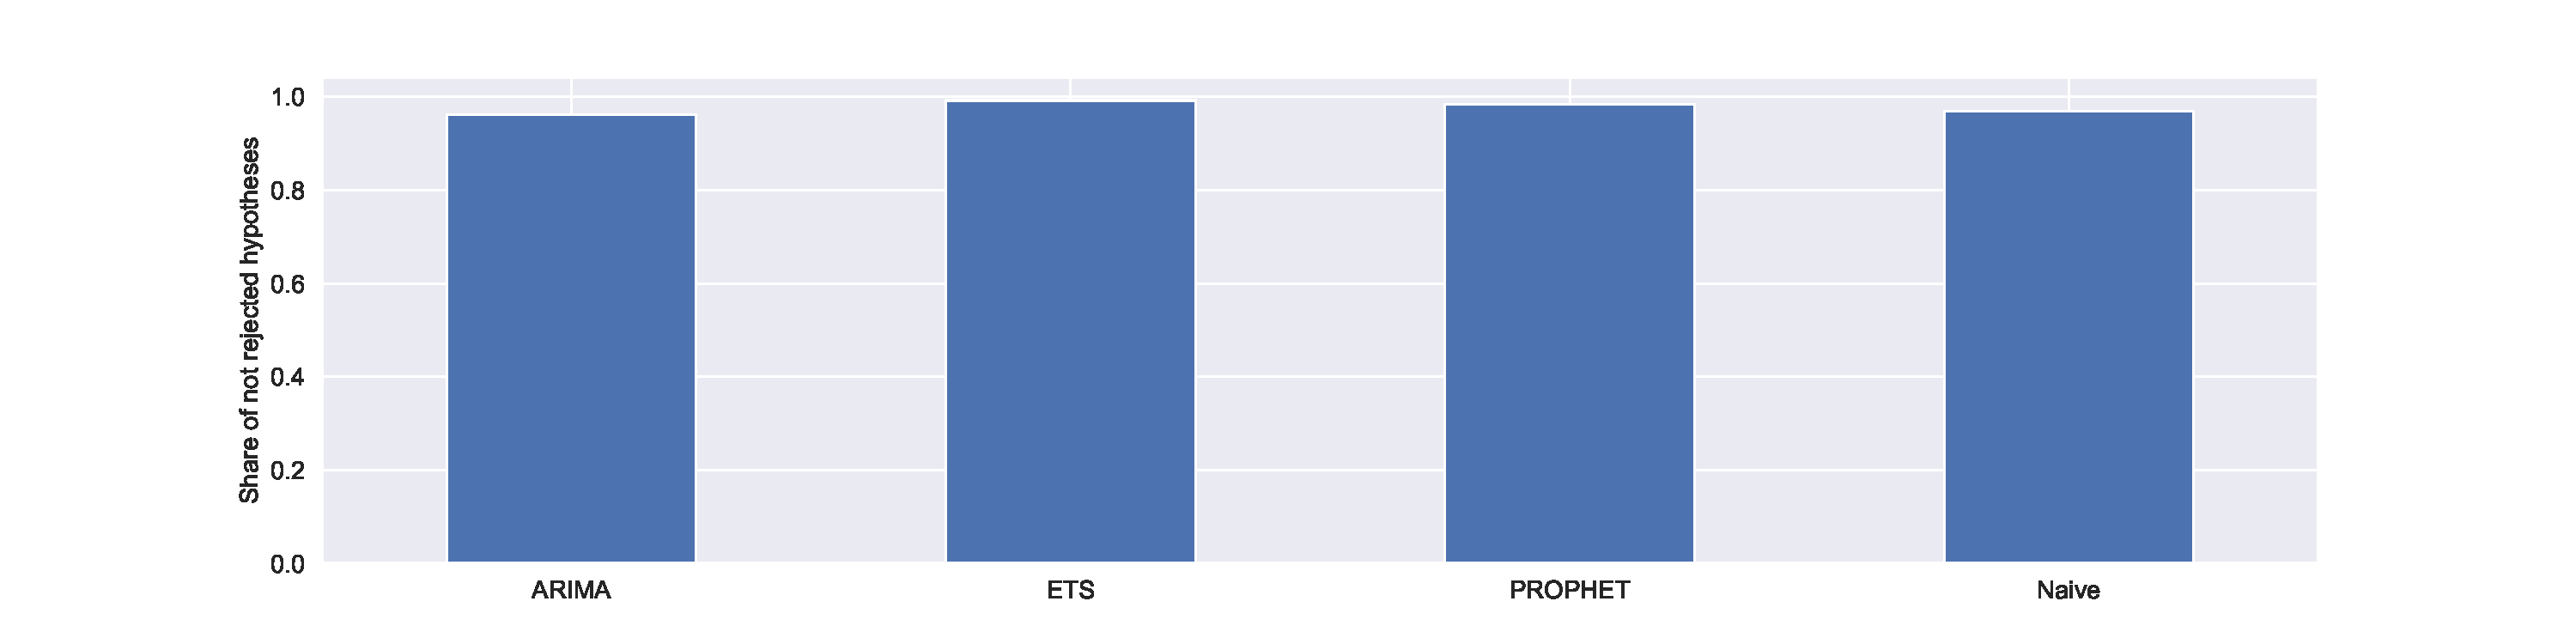
\includegraphics[width=\linewidth]{pictures/results-seasdynreg-full.pdf}
		\caption{Доли неотвергнутых гипотез о том, что cезонная динамическая регрессия не хуже рассматриваемого базового метода}
		\label{results:seasdynreg:full}
	\end{figure}
	Видим, что обе модели имеют большой процент неотвергаемых гипотез, что говорит об успешной работе этих моделей. Рассмотрим теперь сравнение динамических моделей с базовыми методами в зависимости от различных признаков:
	\subsubsection{Периодичность}
	Изобразим столбчатые диаграммы с отдельным измерением периодичности: \ref{results:dynreg:periodicity}, \ref{results:seasdynreg:periodicity}. Мы видим, что общая тенденция сохраняется, но на часовых рядах (вероятно, самых волатильных) качество моделей относительно базовых методов сильно падает. 
	\begin{figure}[!h]
		\captionsetup{justification=centering}
		\centering
		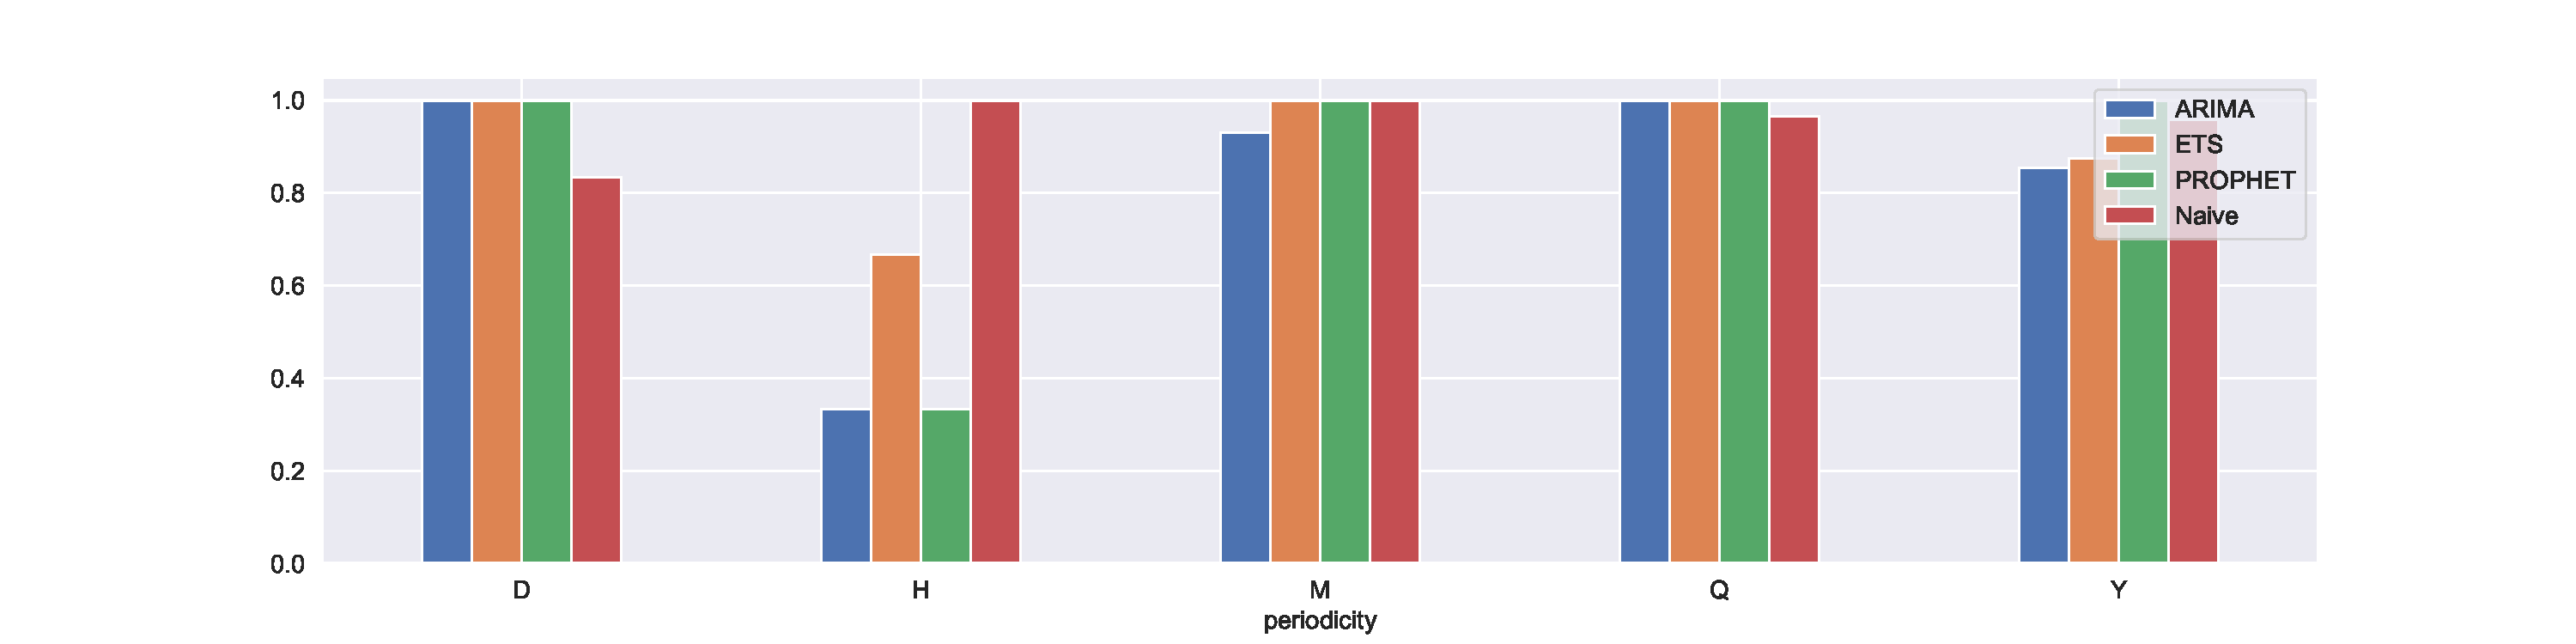
\includegraphics[width=\linewidth]{pictures/results-dynreg-periodicity.pdf}
		\caption{Доли неотвергнутых гипотез о том, что динамическая регрессия \\ не хуже рассматриваемого базового метода \\ в зависимости от периодичности рядов}
		\label{results:dynreg:periodicity}
	\end{figure}
	\begin{figure}[!h]
		\captionsetup{justification=centering}
		\centering
		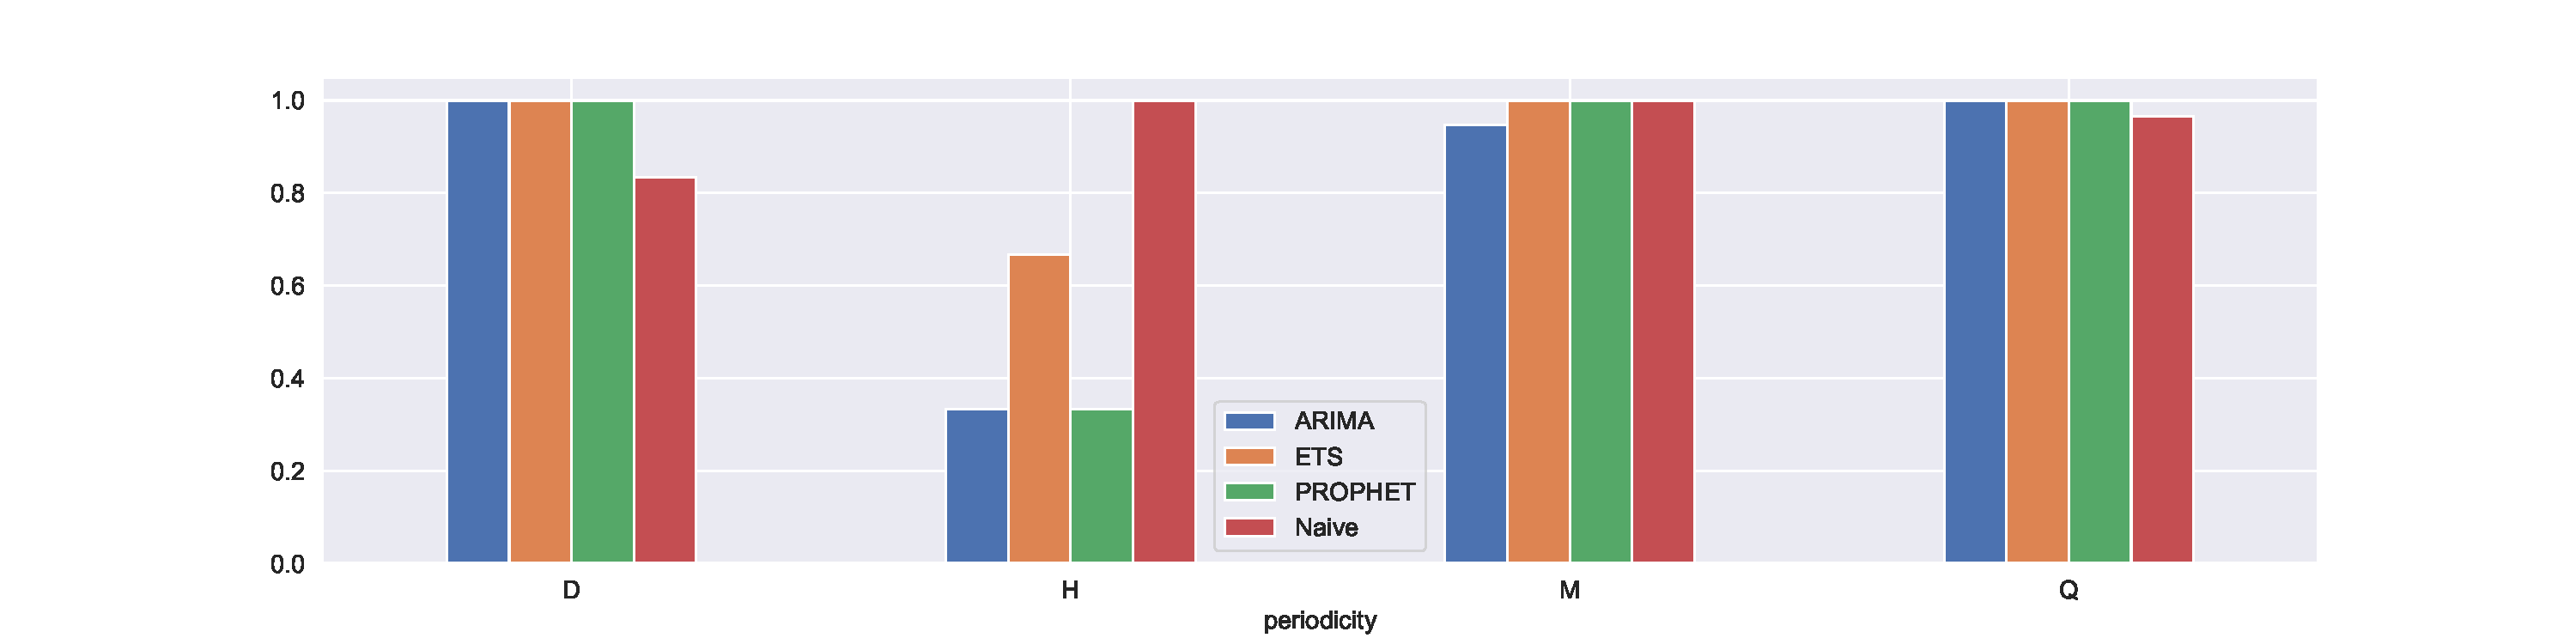
\includegraphics[width=\linewidth]{pictures/results-seasdynreg-periodicity.pdf}
		\caption{Доли неотвергнутых гипотез о том, что cезонная динамическая регрессия не хуже рассматриваемого базового метода \\ в зависимости от периодичности рядов}
		\label{results:seasdynreg:periodicity}
	\end{figure}
	\subsubsection{Категория источника}
	Изобразим графики с отдельным измерением категории источника: \ref{results:dynreg:category}, \ref{results:seasdynreg:category}. Мы видим падение качества по категории Other. Сложно судить, с чем это может быть связано, но одна из гипотез --- достаточно большая часть рядов в категории Other --- часовые, и из-за этого в целом категория более волатильна, чем остальные. Кроме того, можем заметить, что методы ARIMA и ETS примерно в 20\% случаев дают лучшее качество, чем динамические регрессии, на макроэкономических рядах.
	\begin{figure}[!h]
		\captionsetup{justification=centering}
		\centering
		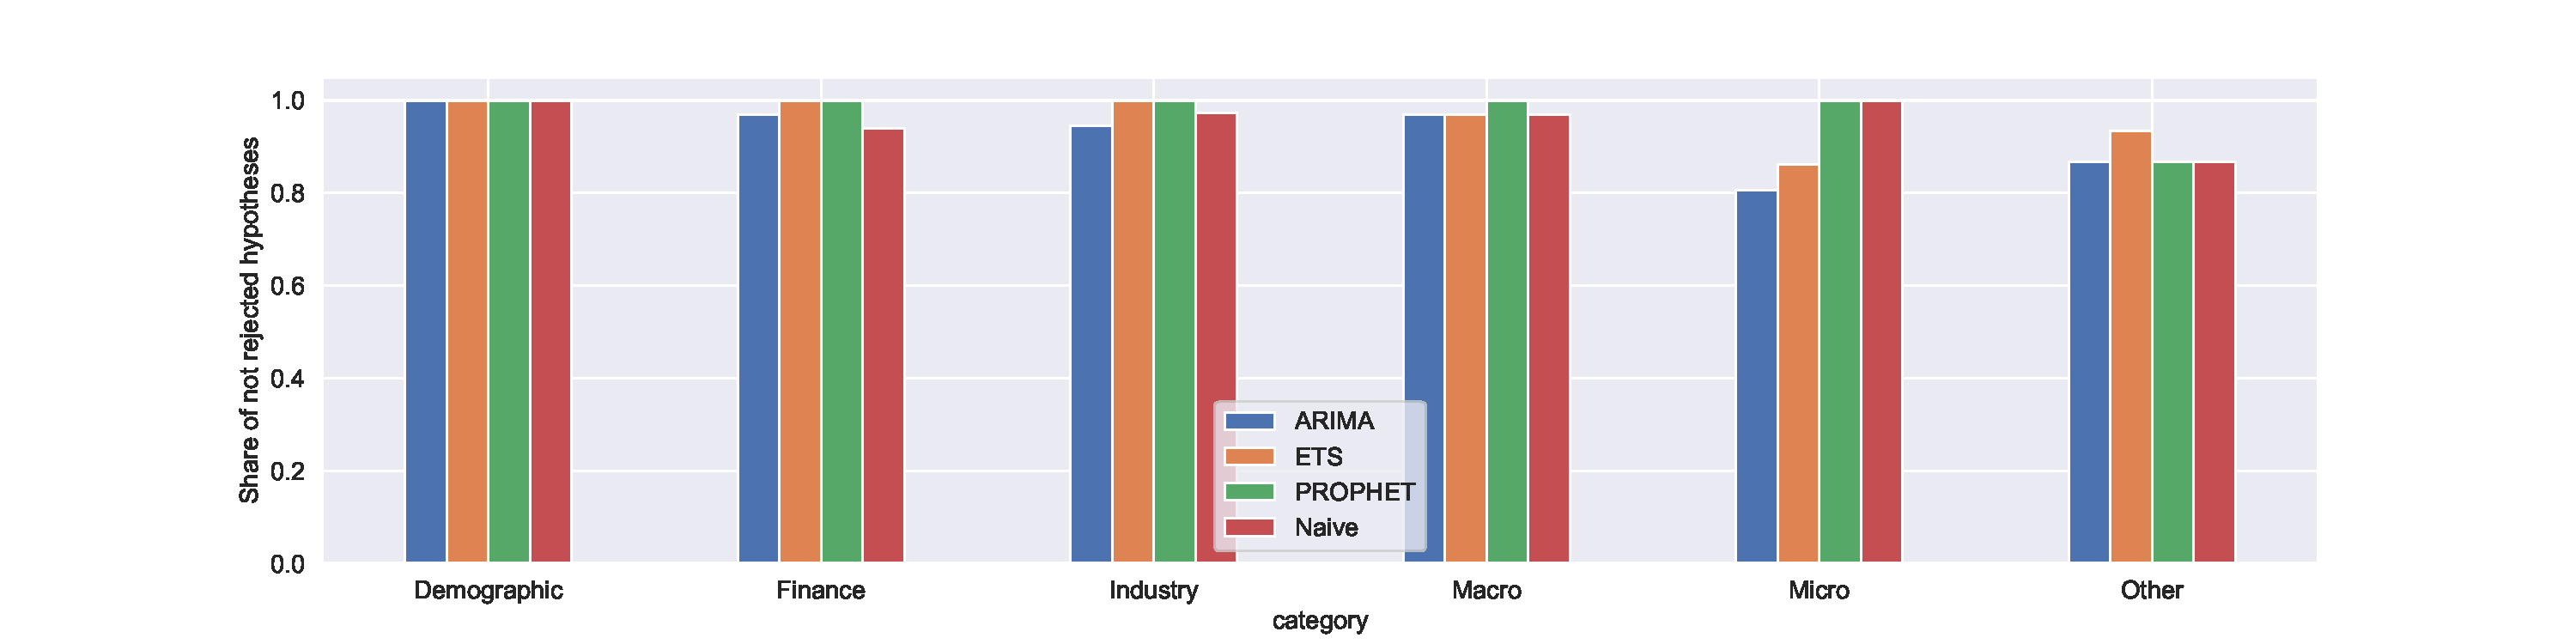
\includegraphics[width=\linewidth]{pictures/results-dynreg-category.pdf}
		\caption{Доли неотвергнутых гипотез о том, что динамическая регрессия \\ не хуже рассматриваемого базового метода \\ в зависимости от категории рядов}
		\label{results:dynreg:category}
	\end{figure}
	\begin{figure}[!h]
		\captionsetup{justification=centering}
		\centering
		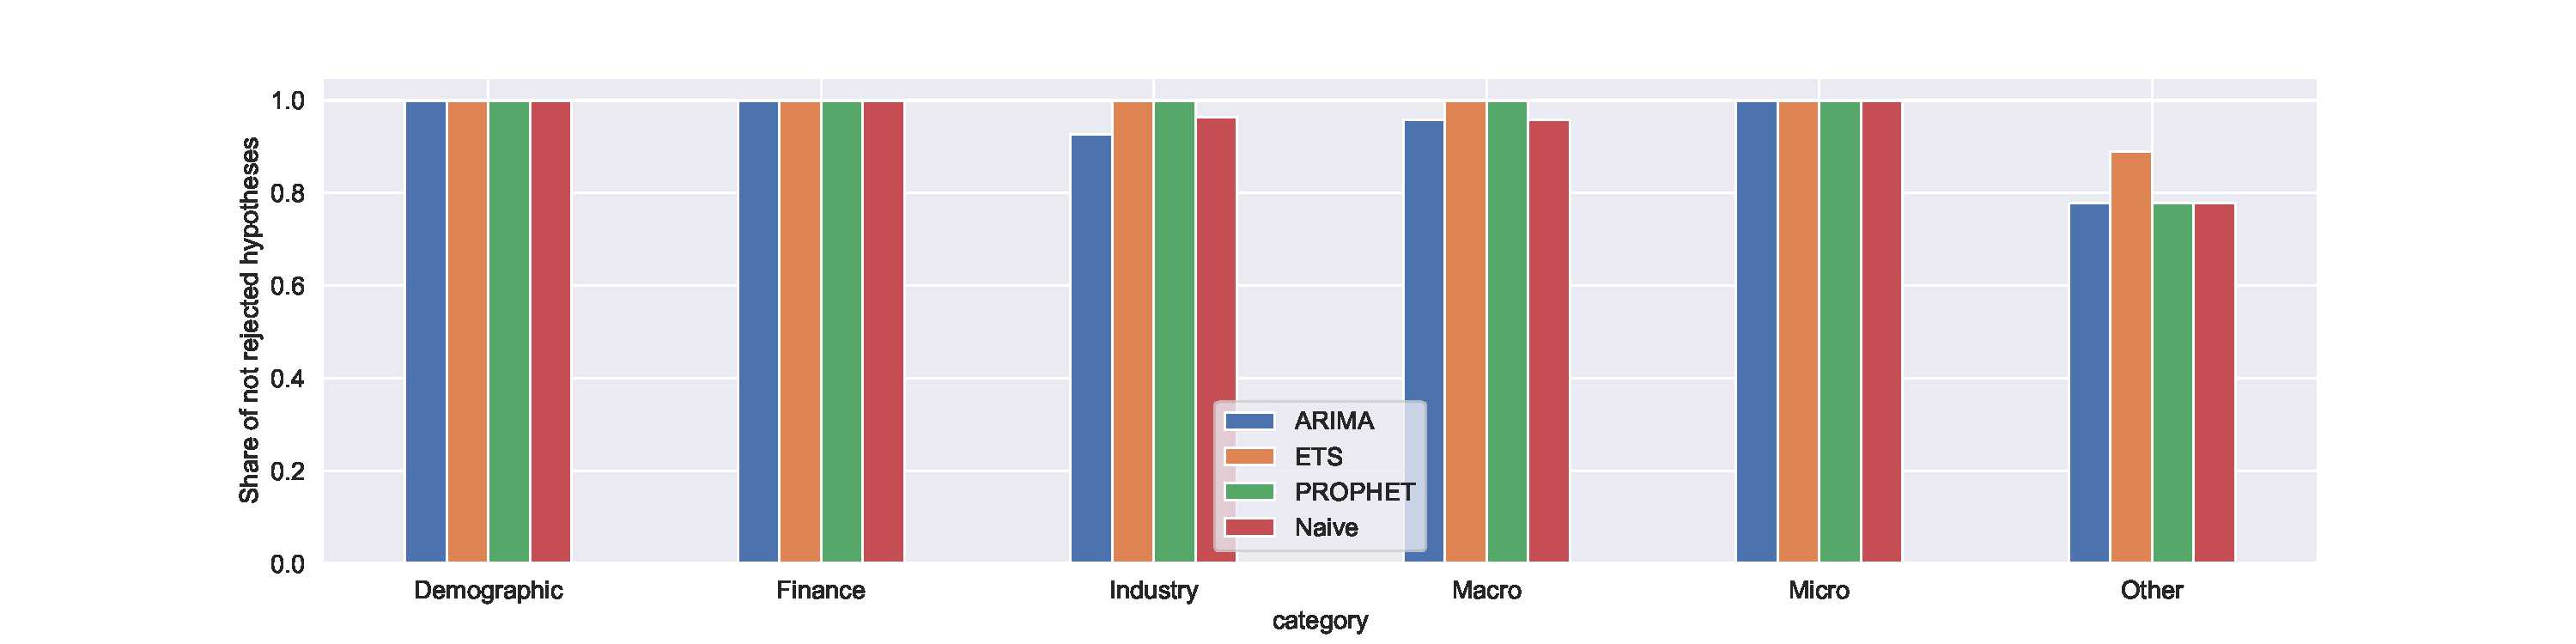
\includegraphics[width=\linewidth]{pictures/results-seasdynreg-category.pdf}
		\caption{Доли неотвергнутых гипотез о том, что cезонная динамическая регрессия не хуже рассматриваемого базового метода \\ в зависимости от категории рядов}
		\label{results:seasdynreg:category}
	\end{figure}
	\subsubsection{Сезонность}
	Нарисуем результаты на рядах в зависимости от сезонности: \ref{results:dynreg:seasonality}, \ref{results:seasdynreg:seasonality}. Наверное, единственное, что выделяется из этого графика --- это то, что на несезонных данных ARIMA начинает работать относительно динамических моделей лучше примерно на 10\%, чем на сезонных. Кроме того, можно отметить, что на сезонных данных сезонная динамическая регрессия статистически оказывается лучше почти всех базовых моделей в 100\% случаях.
	\begin{figure}[!h]
		\captionsetup{justification=centering}
		\centering
		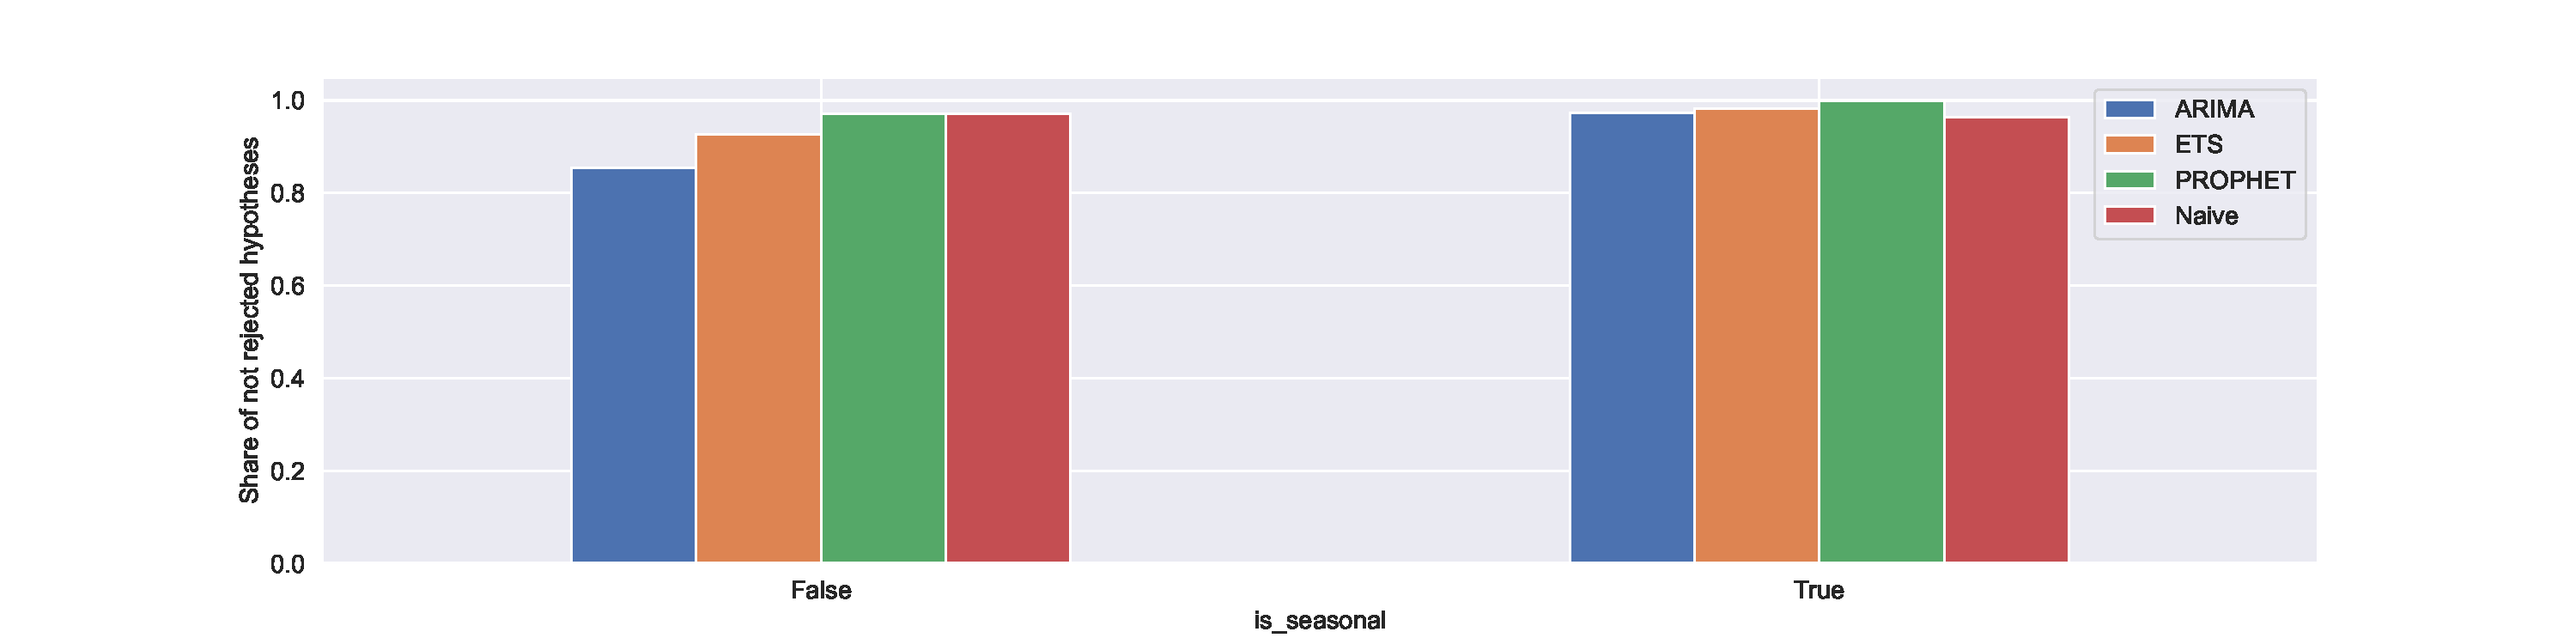
\includegraphics[width=\linewidth]{pictures/results-dynreg-seasonality.pdf}
		\caption{Доли неотвергнутых гипотез о том, что динамическая регрессия \\ не хуже рассматриваемого базового метода \\ в зависимости от сезонности рядов}
		\label{results:dynreg:seasonality}
	\end{figure}
	\begin{figure}[!h]
		\captionsetup{justification=centering}
		\centering
		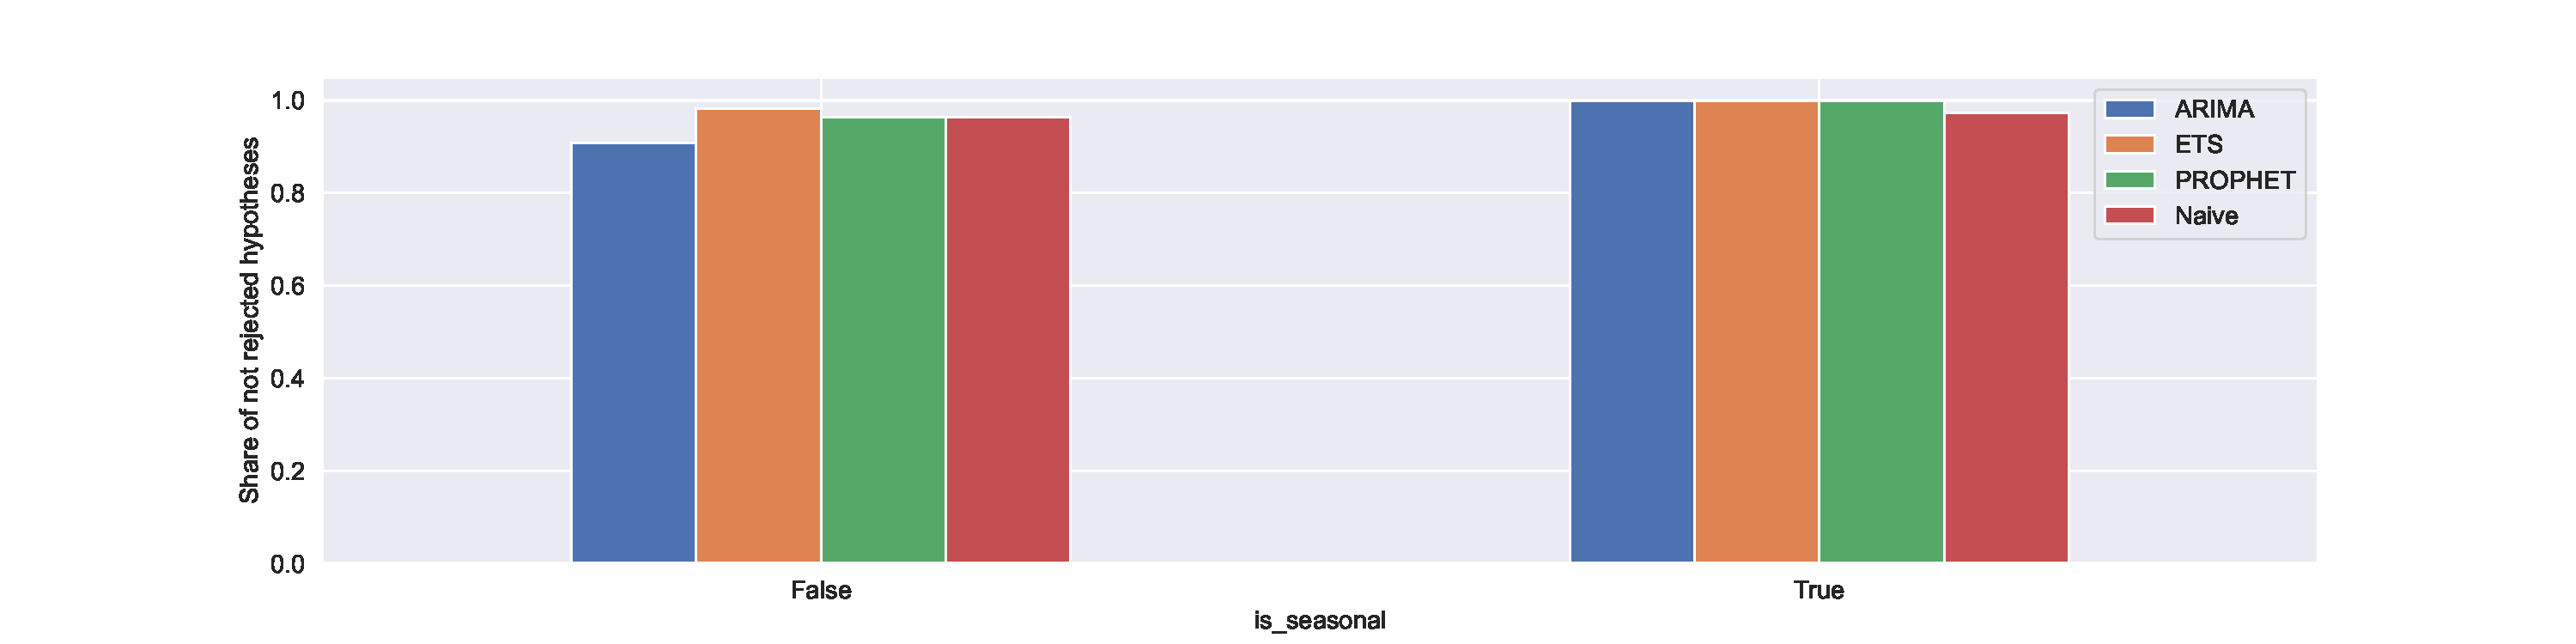
\includegraphics[width=\linewidth]{pictures/results-seasdynreg-seasonality.pdf}
		\caption{Доли неотвергнутых гипотез о том, что cезонная динамическая регрессия не хуже рассматриваемого базового метода \\ в зависимости от сезонности рядов}
		\label{results:seasdynreg:seasonality}
	\end{figure}
	\subsubsection{Стационарность}
	Изобразим графики с отдельным измерением стационарности: \ref{results:dynreg:stationary}, \ref{results:seasdynreg:stationary}. На мой взгляд, между двумя диаграммами больших изменений нет. Как в случае стационарных рядов, так и в случае нестационарных, динамические модели почти всегда работают не хуже базовых методов.
	\begin{figure}[!h]
		\captionsetup{justification=centering}
		\centering
		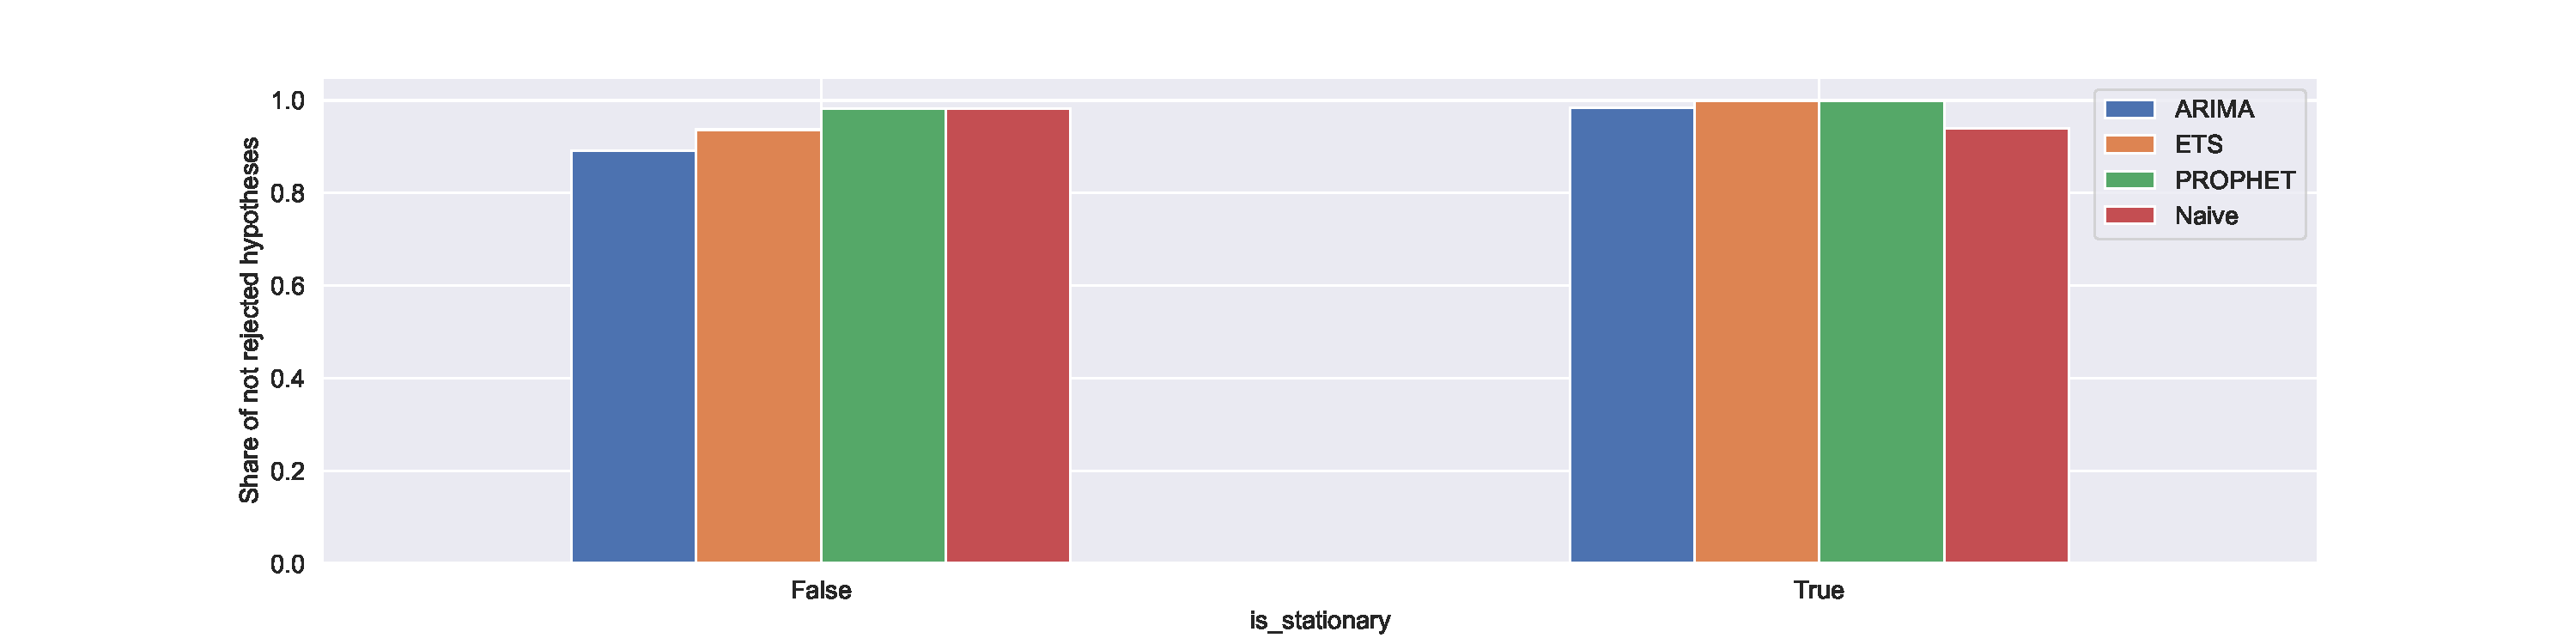
\includegraphics[width=\linewidth]{pictures/results-dynreg-stationarity.pdf}
		\caption{Доли неотвергнутых гипотез о том, что динамическая регрессия \\ не хуже рассматриваемого базового метода \\ в зависимости от стационарности рядов}
		\label{results:dynreg:stationary}
	\end{figure}
	\begin{figure}[!h]
		\captionsetup{justification=centering}
		\centering
		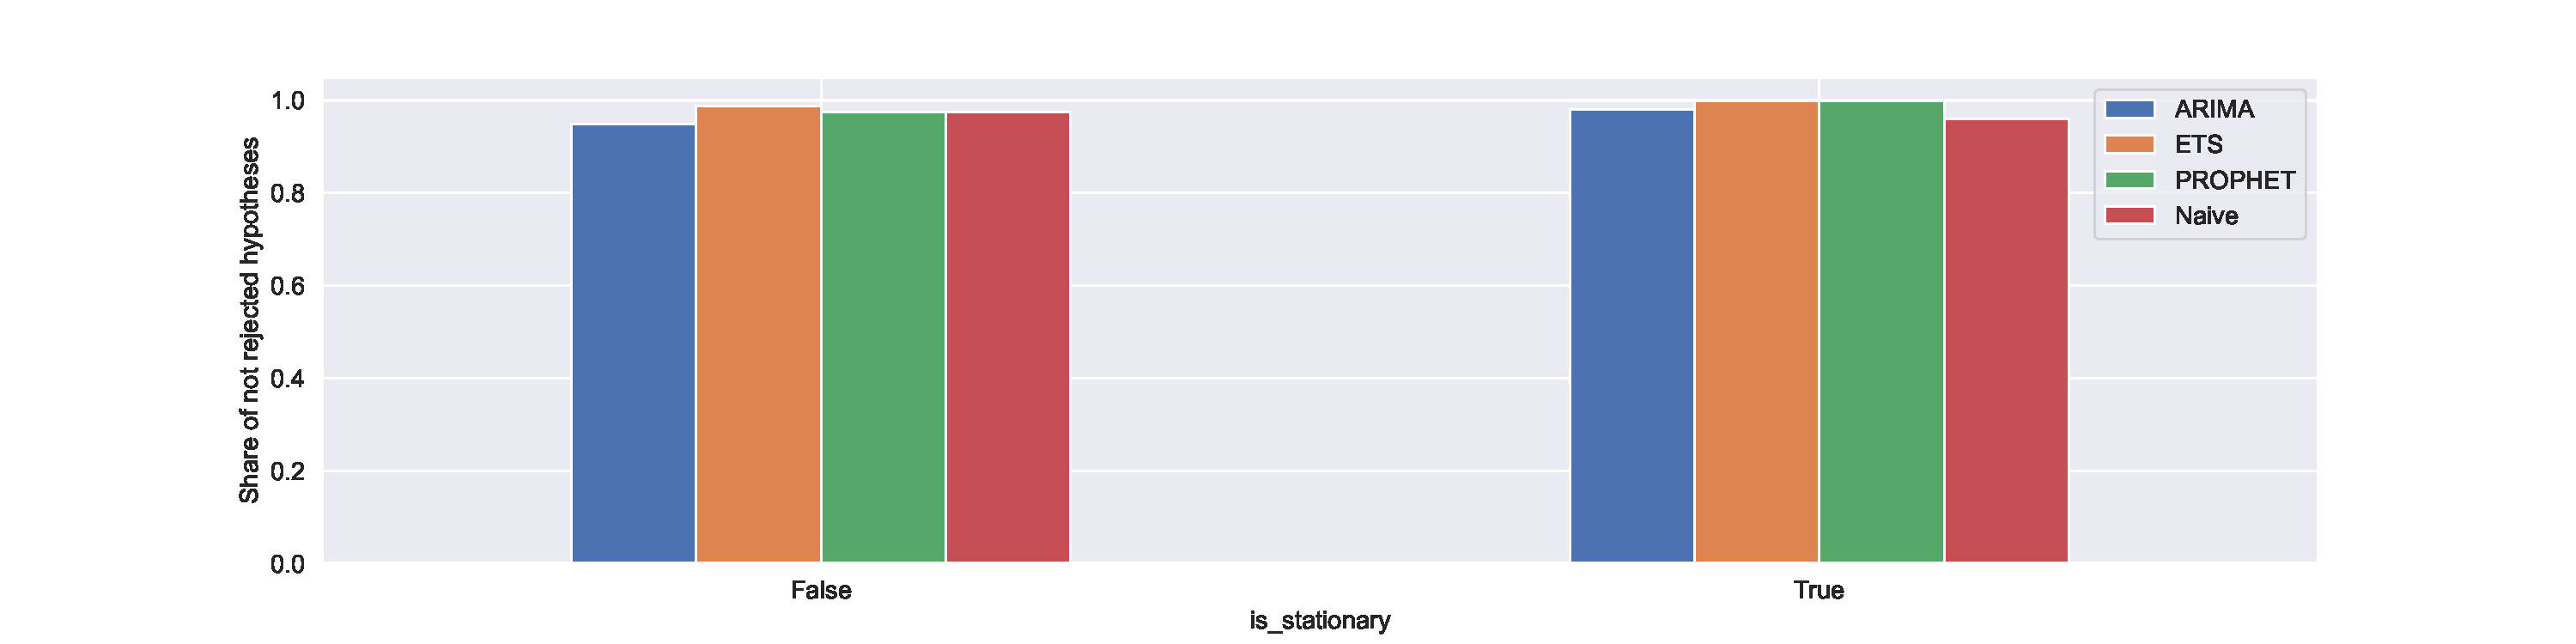
\includegraphics[width=\linewidth]{pictures/results-seasdynreg-stationarity.pdf}
		\caption{Доли неотвергнутых гипотез о том, что cезонная динамическая регрессия не хуже рассматриваемого базового метода \\ в зависимости от стационарности рядов}
		\label{results:seasdynreg:stationary}
	\end{figure}
	\subsubsection{Горизонт прогнозирования}
	Нарисуем графики с отдельным измерением для горизонта прогнозирования: \ref{results:dynreg:fh}, \ref{results:seasdynreg:fh}. На обоих графиках мы видим, что лучшие результаты относительно базовых методов динамические модели показывают именно на дальнем шаге. При этом хуже всего они работают, если нужно до этого дальнего шага спрогнозировать весь путь. 
	\begin{figure}[!h]
		\captionsetup{justification=centering}
		\centering
		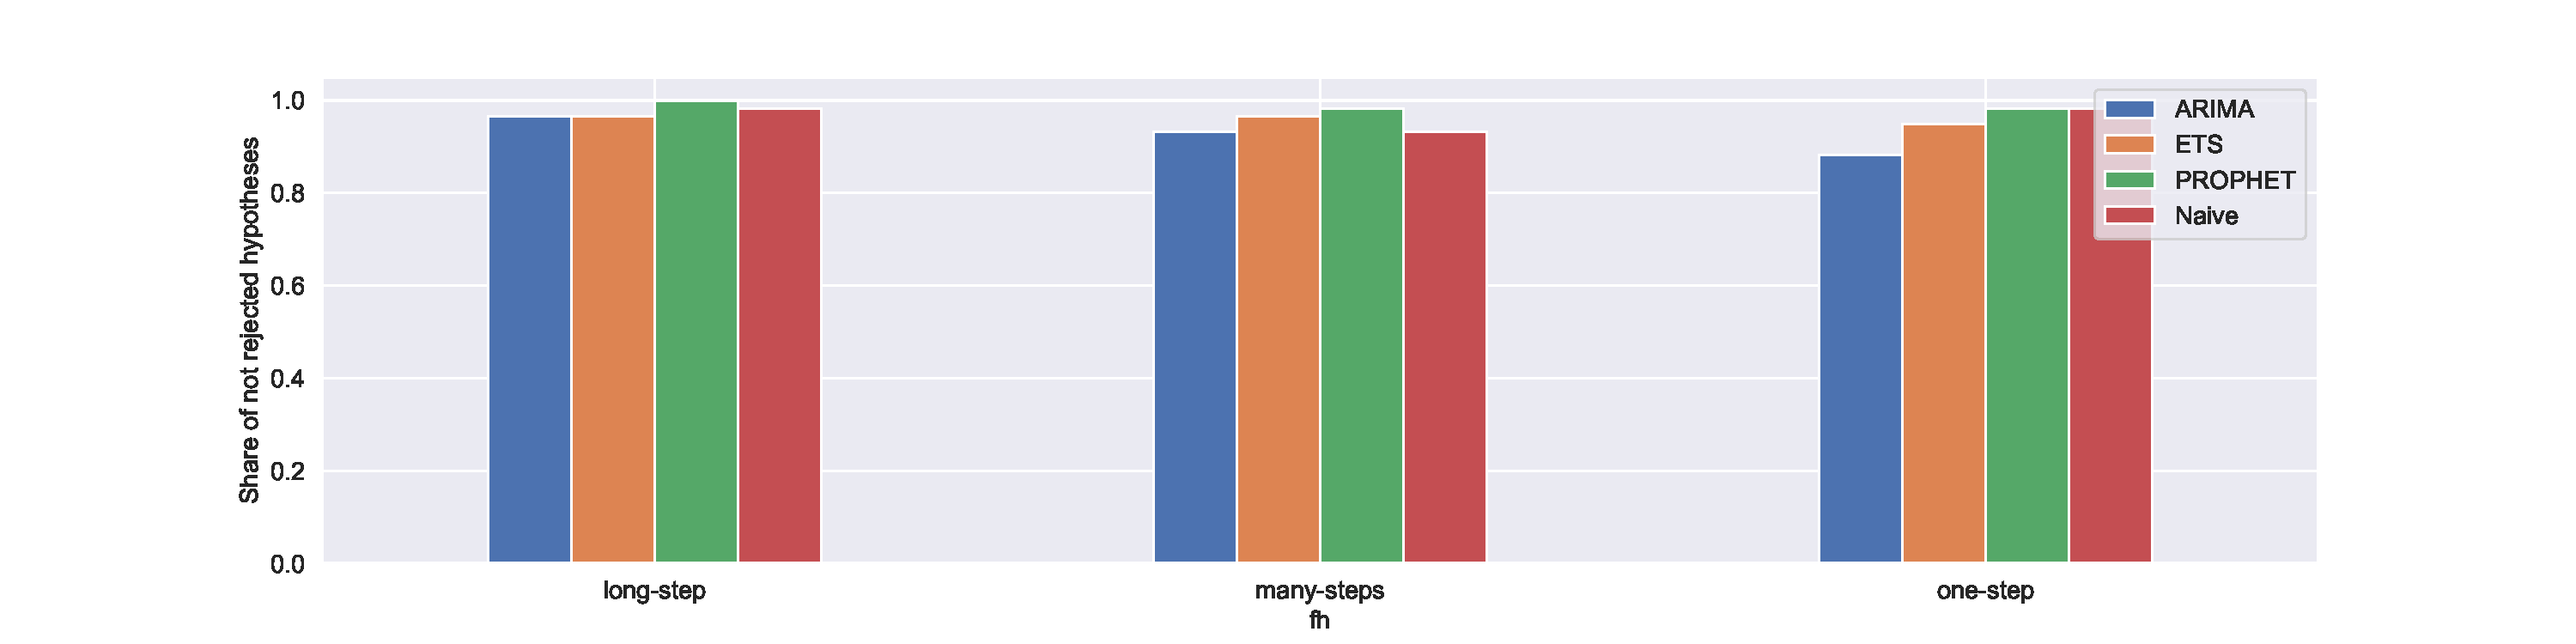
\includegraphics[width=\linewidth]{pictures/results-dynreg-fh.pdf}
		\caption{Доли неотвергнутых гипотез о том, что динамическая регрессия \\ не хуже рассматриваемого базового метода \\ в зависимости от горизонта прогнозирования}
		\label{results:dynreg:fh}
	\end{figure}
	\begin{figure}[!h]
		\captionsetup{justification=centering}
		\centering
		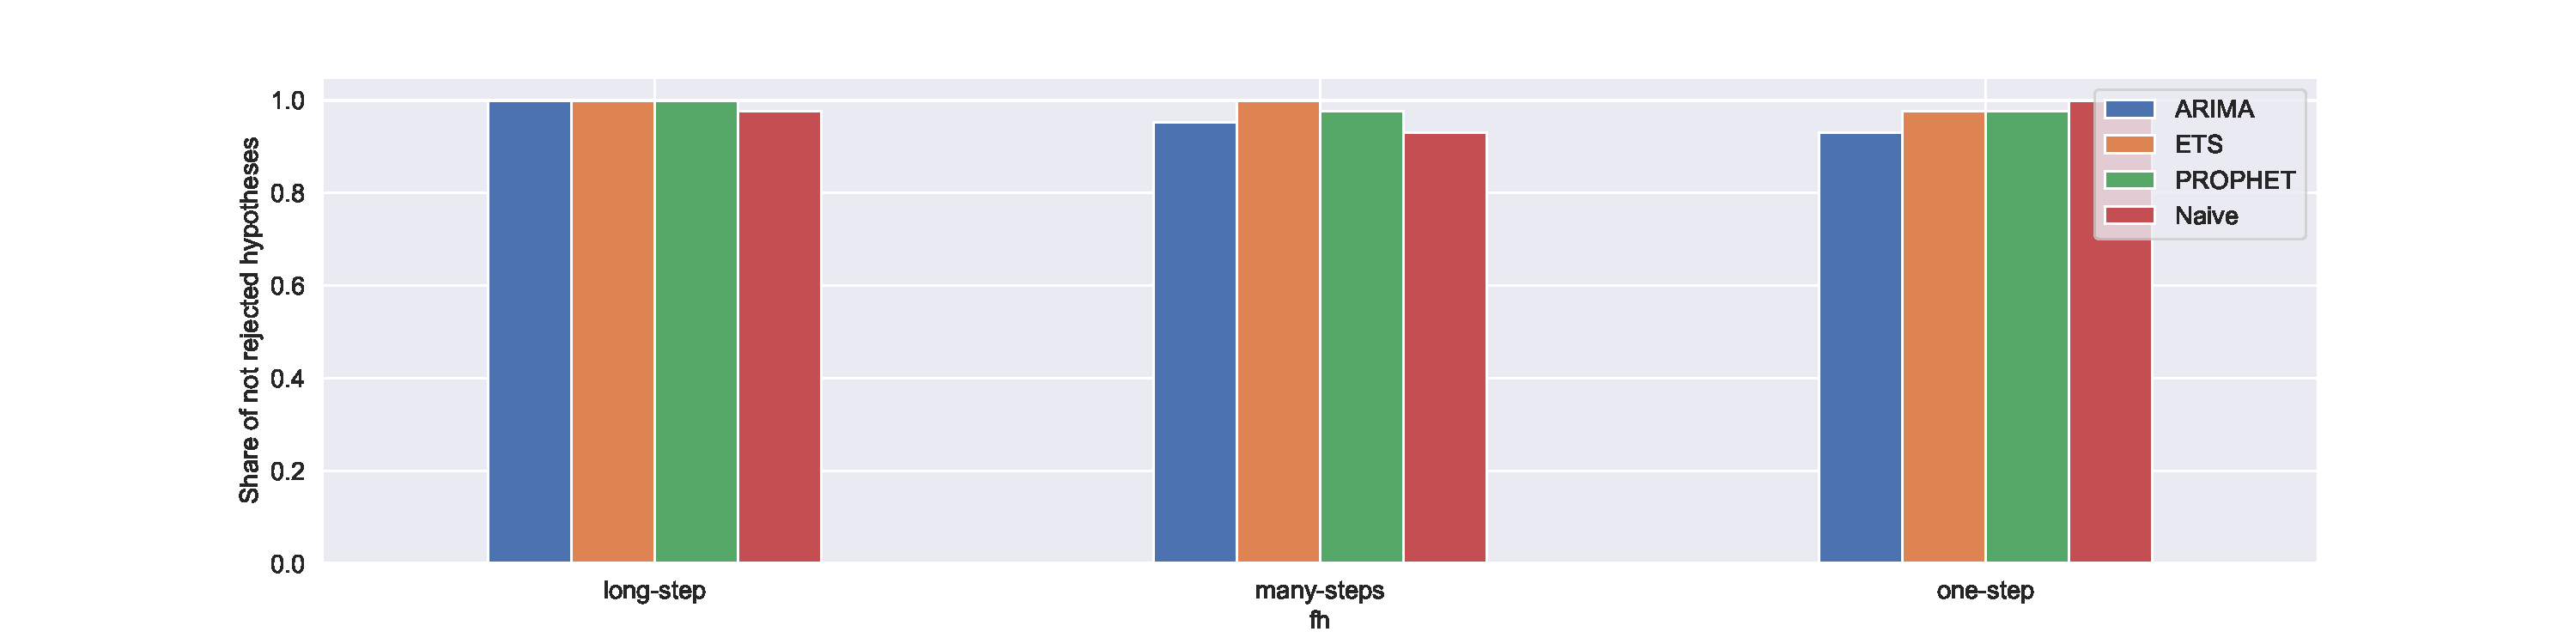
\includegraphics[width=\linewidth]{pictures/results-seasdynreg-fh.pdf}
		\caption{Доли неотвергнутых гипотез о том, что cезонная динамическая регрессия не хуже рассматриваемого базового метода \\ в зависимости от горизонта прогнозирования}
		\label{results:seasdynreg:fh}
	\end{figure}

	\newpage
	\newpage

	Таким образом, во всех рассмотренных случаях динамические модели работают в основном не хуже, чем рассмотренные базовые методы. 
	\subsection{Выявление благоприятных временных рядов}
	Теперь постараемся найти свойства временных рядов, на которых динамические модели справляются лучше не какой-то конкретной модели, а сразу всех моделей в целом. Для этого мы будем для каждого множества кластеров изображать круговую диаграмму с процентом побед для каждой модели. Начнём с круговой диаграммы по всем кластерам: \ref{wins:full}.
	\begin{figure}[!h]
		\captionsetup{justification=centering}
		\centering
		
\includegraphics[width=\linewidth]{pictures/wins-full.pdf}
		\caption{Проценты побед рассматриваемых моделей}
		\label{wins:full}
	\end{figure}
	На данной диаграмме примерно 30\% побед у сезонной динамической регрессии, и таким образом её можно признать самой сильной моделью из рассмотренных. У обычной динамической регрессии на всех кластерах около 23\% побед, что тоже является достойным показателем. Рассмотрим более подробно влияние различных признаков на качество реализованных моделей:
	\subsubsection{Периодичность}
	Изобразим проценты побед в зависимости от периодичности рядов: \ref{wins:periodicity}. На графике мы видим, что периодичность может повлиять на качество таких моделей: на часовых данных они начинают работать хуже относительно в основном модели PROPHET. Самую стабильную работу на изображённом графике можно видеть при дневных, квартальных и годовых данных.
	\begin{figure}[!h]
		\captionsetup{justification=centering}
		\centering
		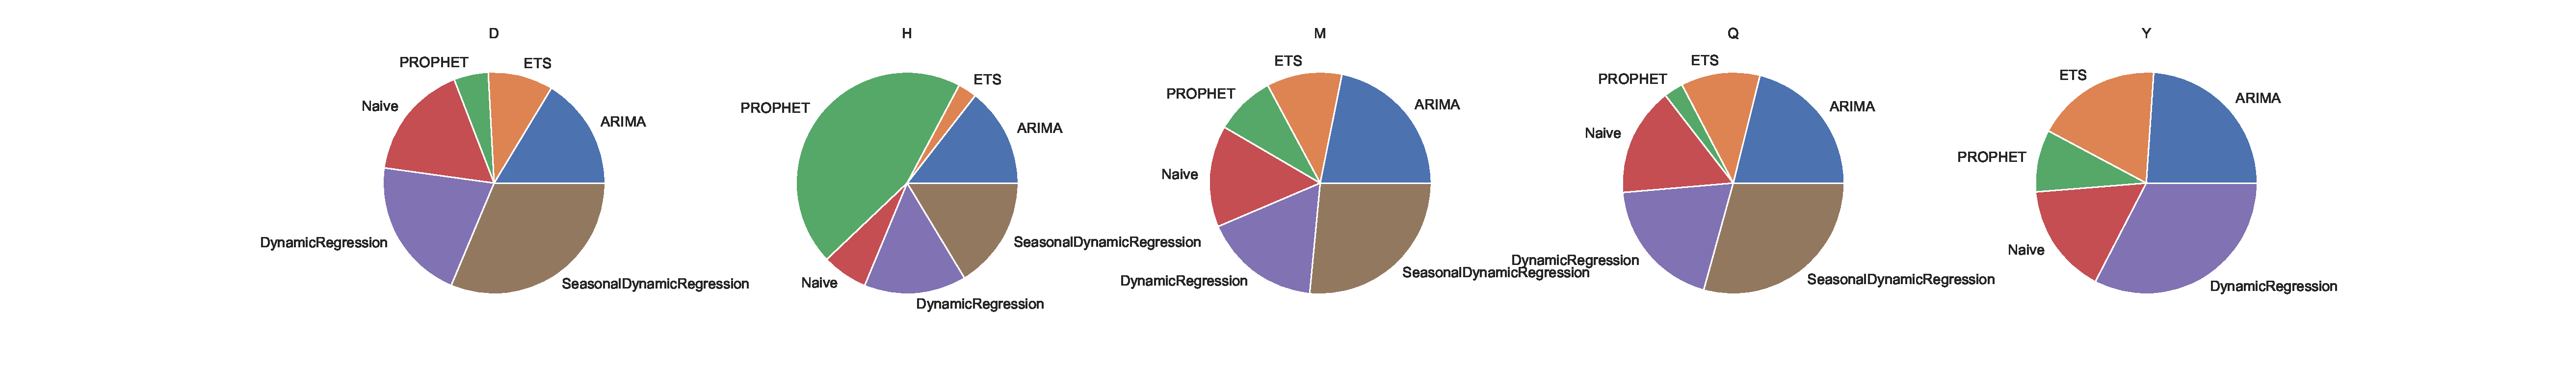
\includegraphics[width=\linewidth]{pictures/wins-periodicity.pdf}
		\caption{Проценты побед рассматриваемых моделей в зависимости от периодичности рядов}
		\label{wins:periodicity}
	\end{figure}
	\subsubsection{Категория источника}
	Нарисуем результаты в зависимости от категории рядов: \ref{wins:category}. Мы видим, что корреляции между источниками данных и особенностями работы динамических моделей не обнаруживается.
	\begin{figure}[!h]
		\captionsetup{justification=centering}
		\centering
		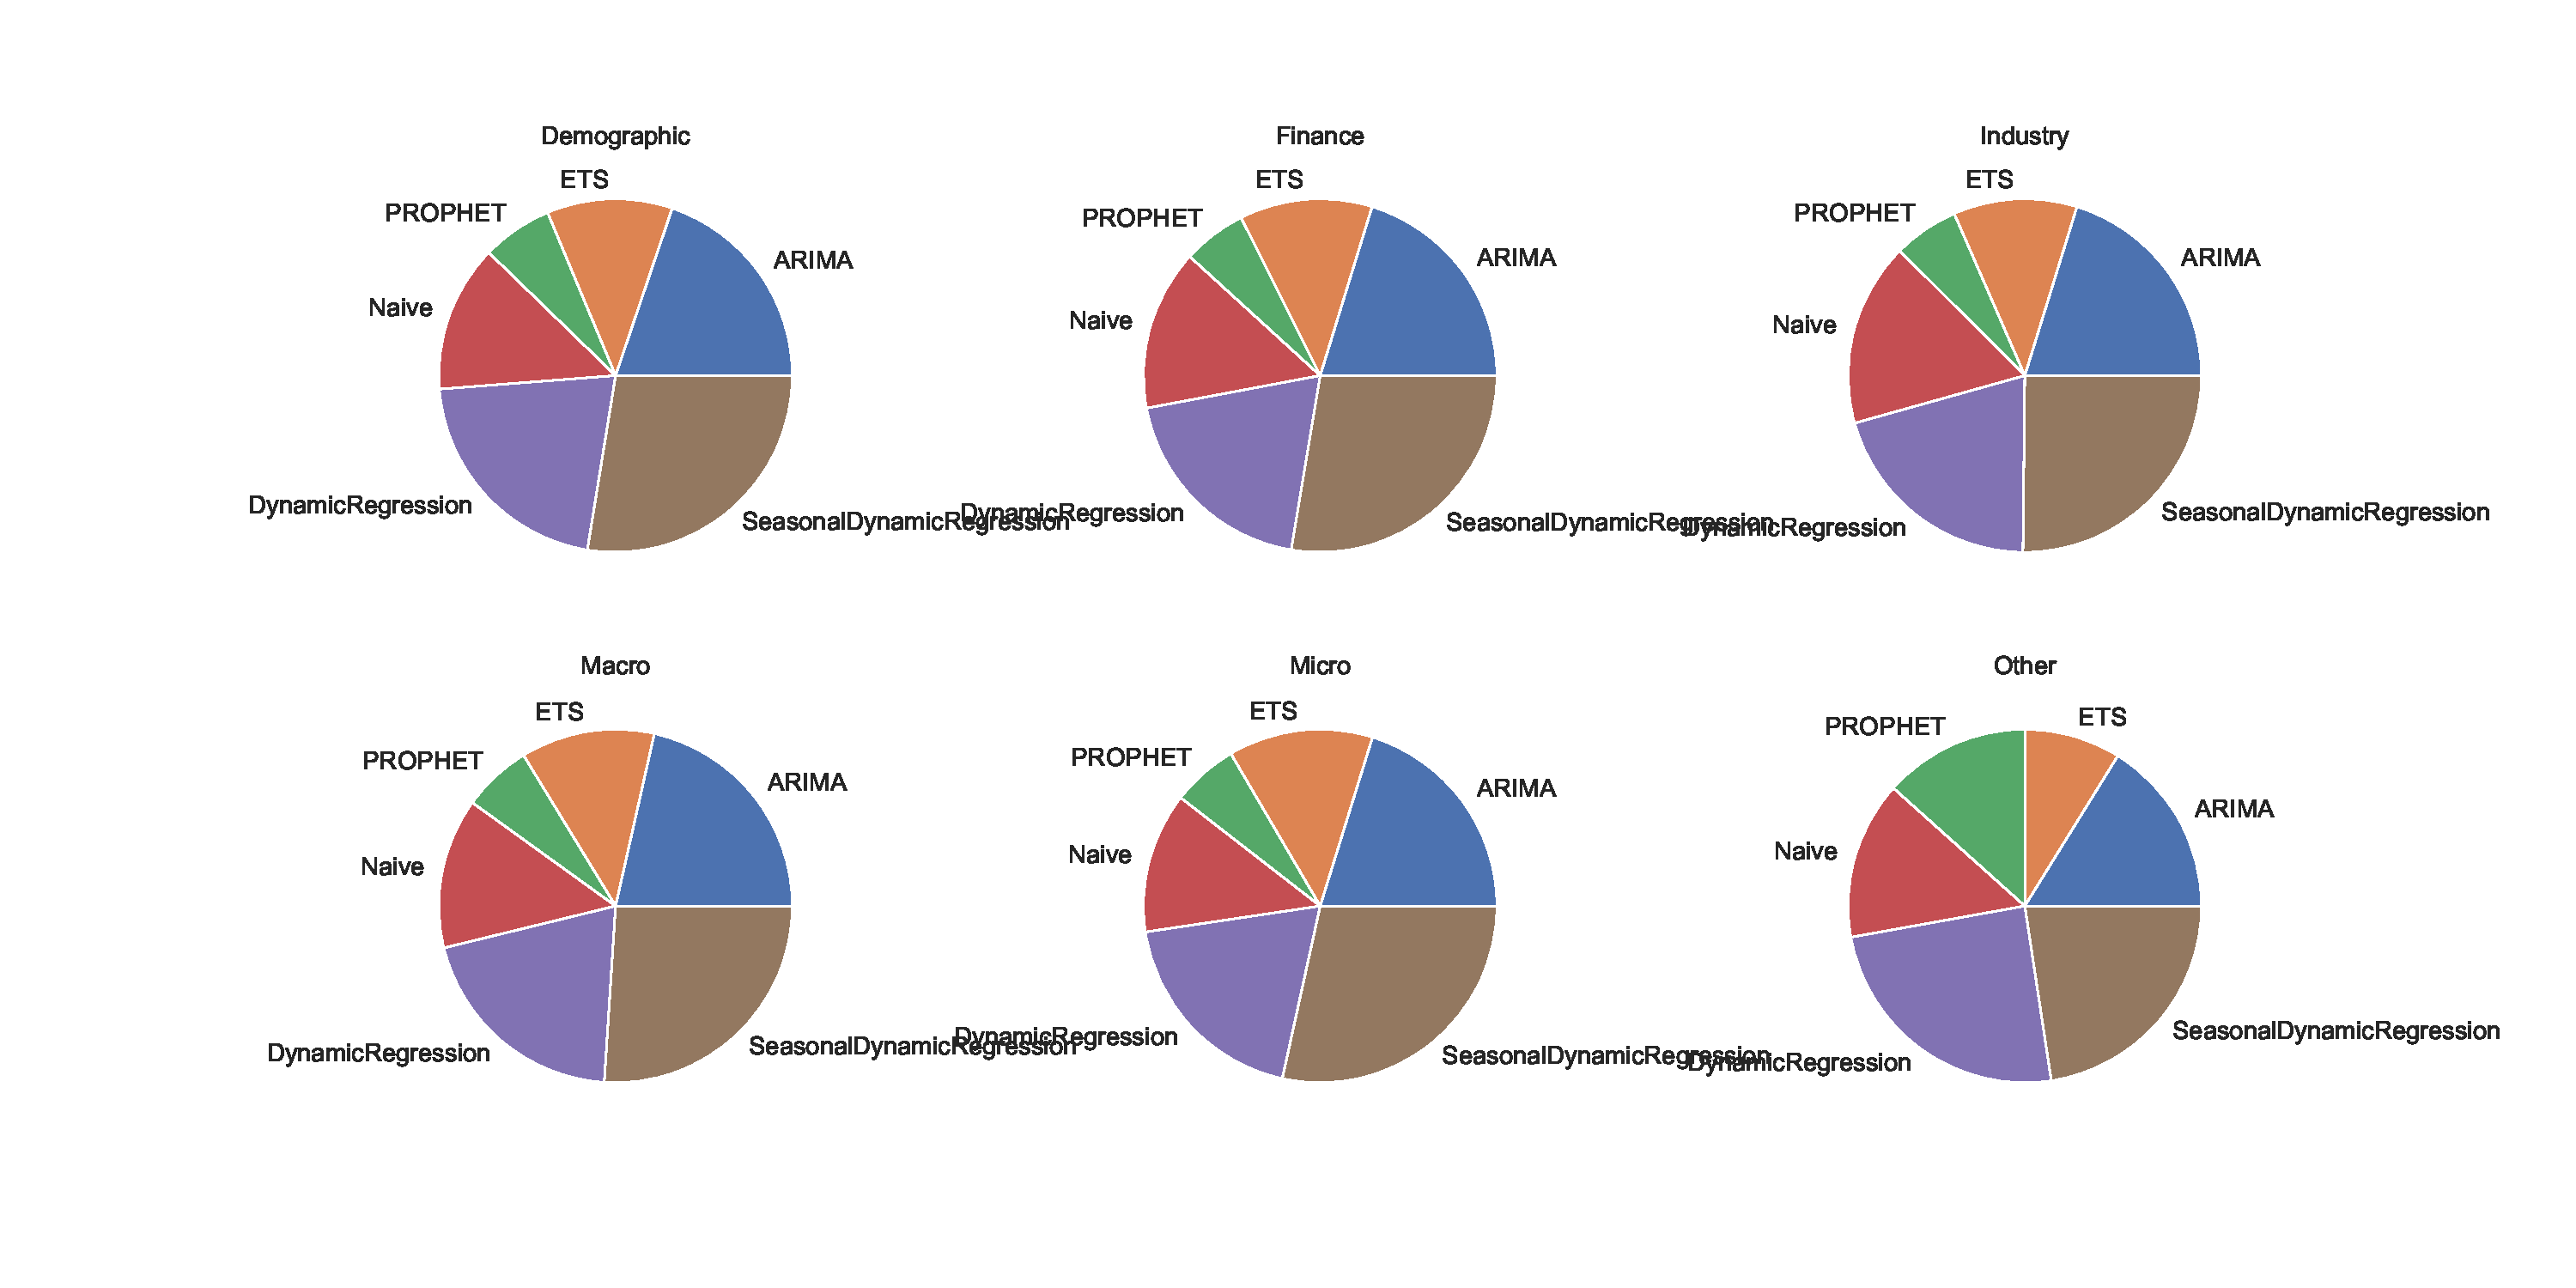
\includegraphics[width=\linewidth]{pictures/wins-category.pdf}
		\caption{Проценты побед рассматриваемых моделей в зависимости от категории рядов}
		\label{wins:category}
	\end{figure}
	\subsubsection{Сезонность}
	Выведем графики процента побед моделей в зависимости от сезонности рядов: \ref{wins:seasonality}. Мы действительно видим, что в случае сезонности обрабатываемых рядов качество динамических моделей вырастает до 50\% побед совместно у динамической и сезонной динамической регрессий. Таким образом, этот фактор может повлиять на качество прогнозов.
	\begin{figure}[!h]
		\captionsetup{justification=centering}
		\centering
		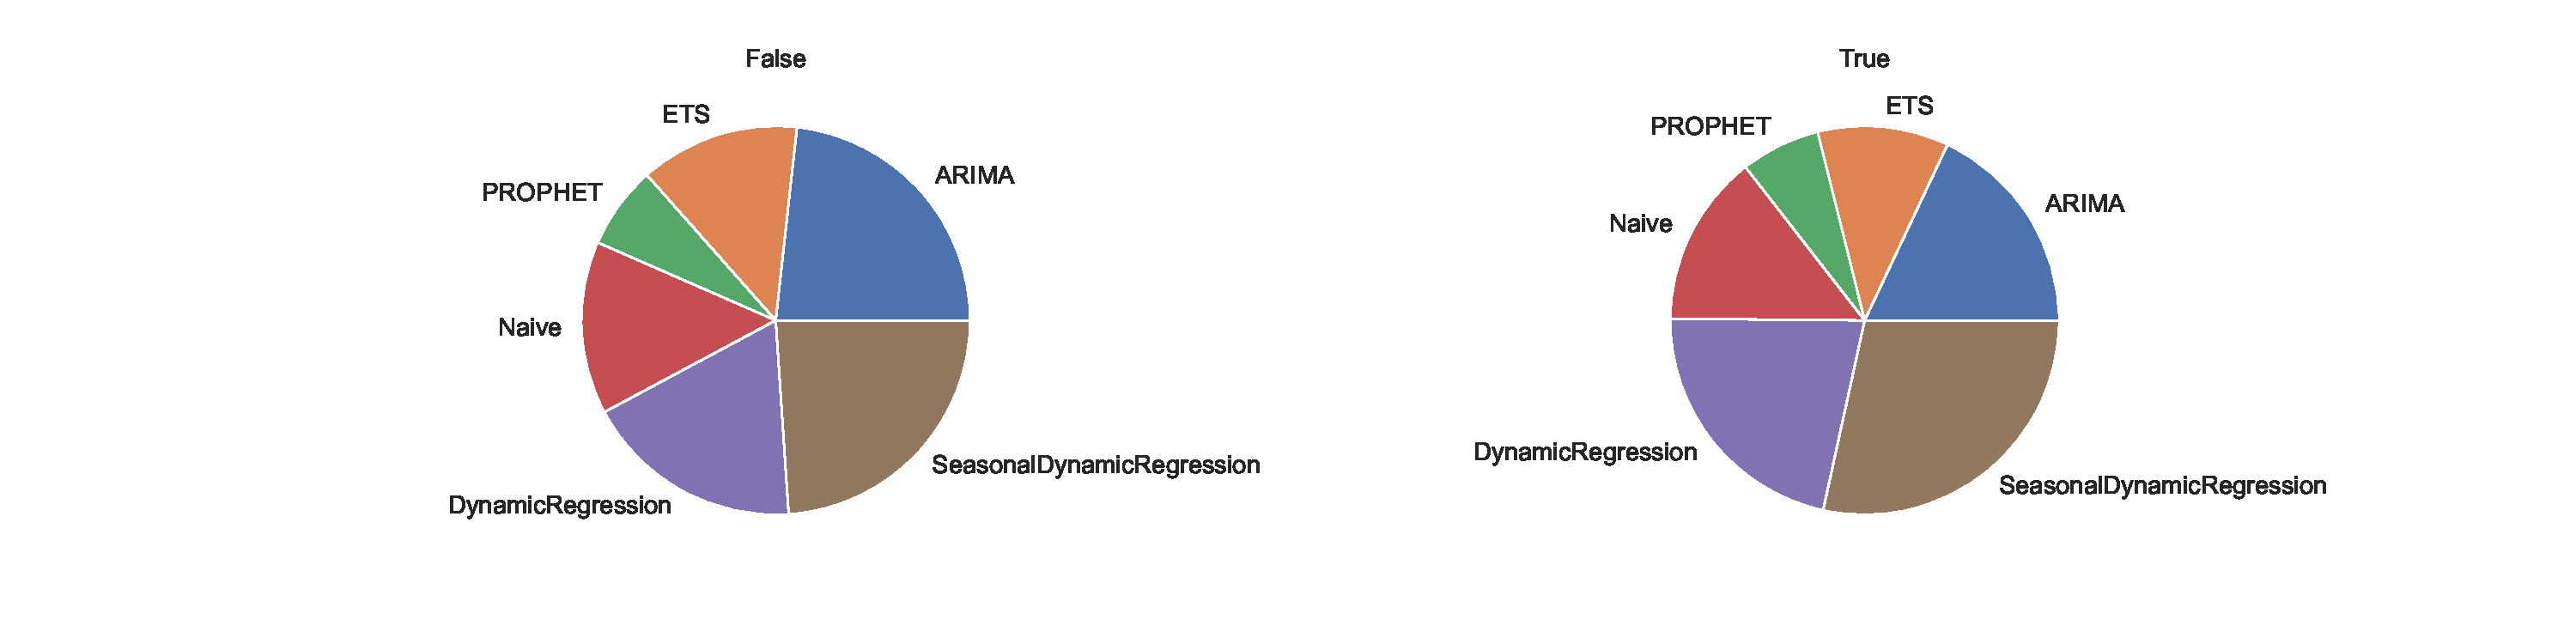
\includegraphics[width=\linewidth]{pictures/wins-seasonality.pdf}
		\caption{Проценты побед рассматриваемых моделей в зависимости от сезонности рядов}
		\label{wins:seasonality}
	\end{figure}
	\subsubsection{Стационарность}
	Изобразим результаты с разделением по стационарности: \ref{wins:stationary}. Мы видим, что этот фактор очень слабо влияет на качество динамических моделей, так как две диаграммы практически одинаковы.
	\begin{figure}[!h]
		\captionsetup{justification=centering}
		\centering
		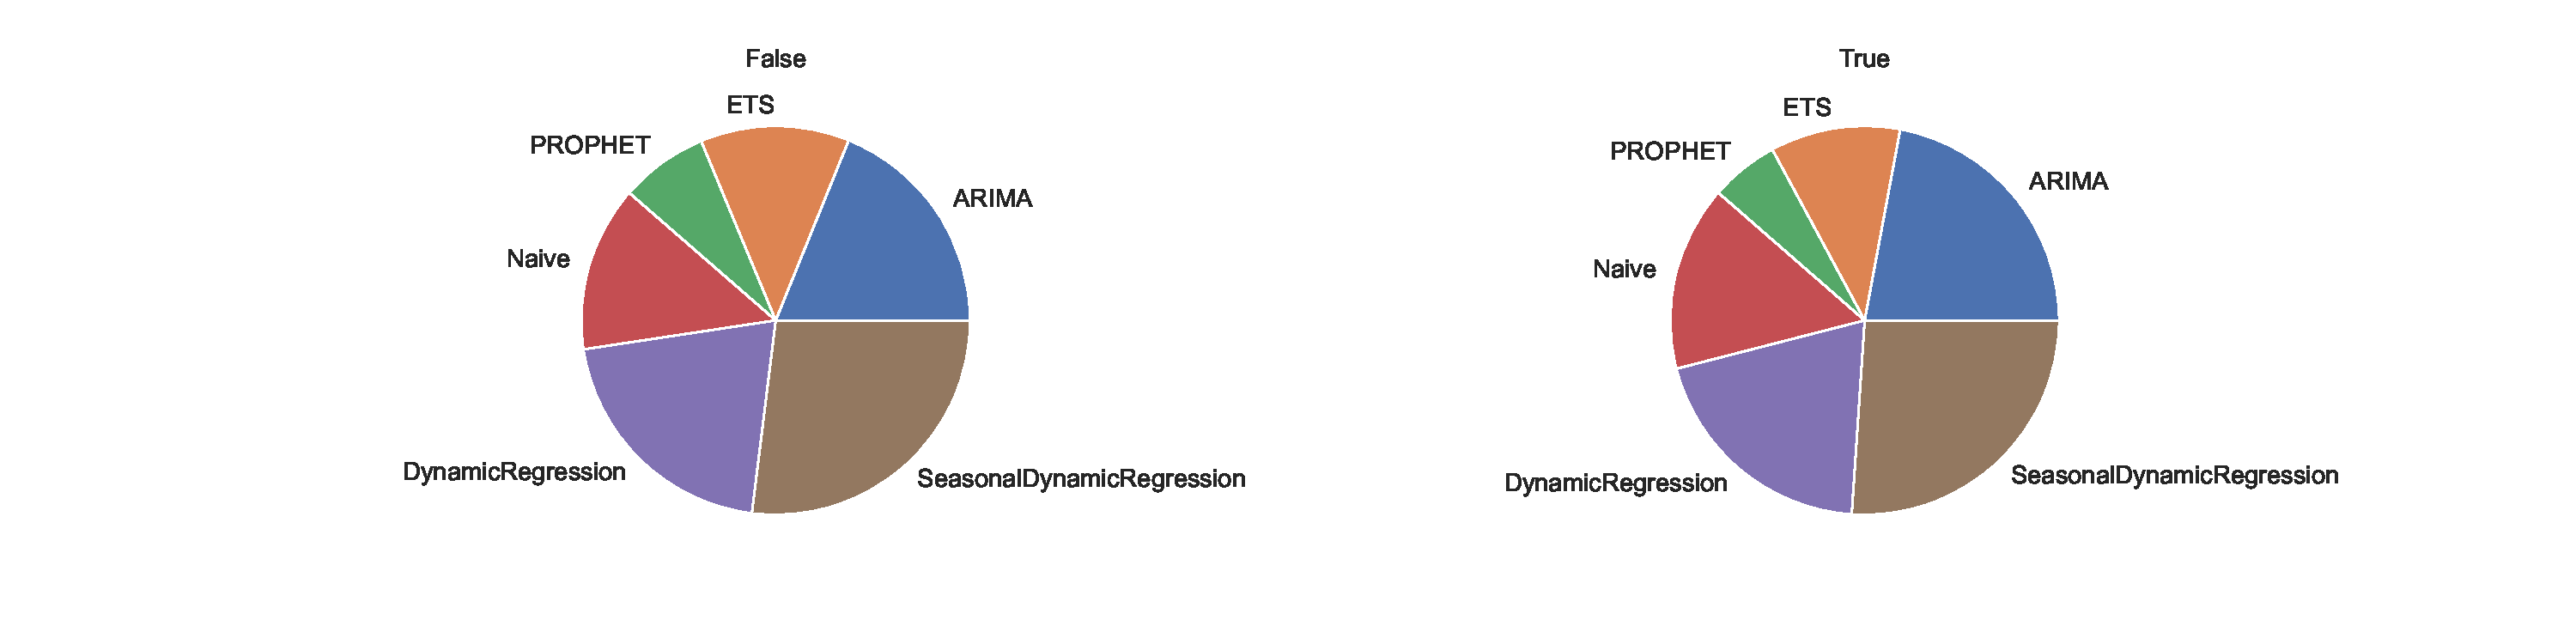
\includegraphics[width=\linewidth]{pictures/wins-stationarity.pdf}
		\caption{Проценты побед рассматриваемых моделей в зависимости от стационарности рядов}
		\label{wins:stationary}
	\end{figure}
	\subsubsection{Горизонт прогнозирования}
	Наконец, покажем работу моделей относительно горизонта прогнозирования: \ref{wins:fh}. Мы видим, что хуже всего динамические модели справляются спрогнозировать весь путь до дальнего шага, а лучше всего получается прогнозировать на один шаг с больше чем 50\% побед.
	\begin{figure}[!h]
		\captionsetup{justification=centering}
		\centering
		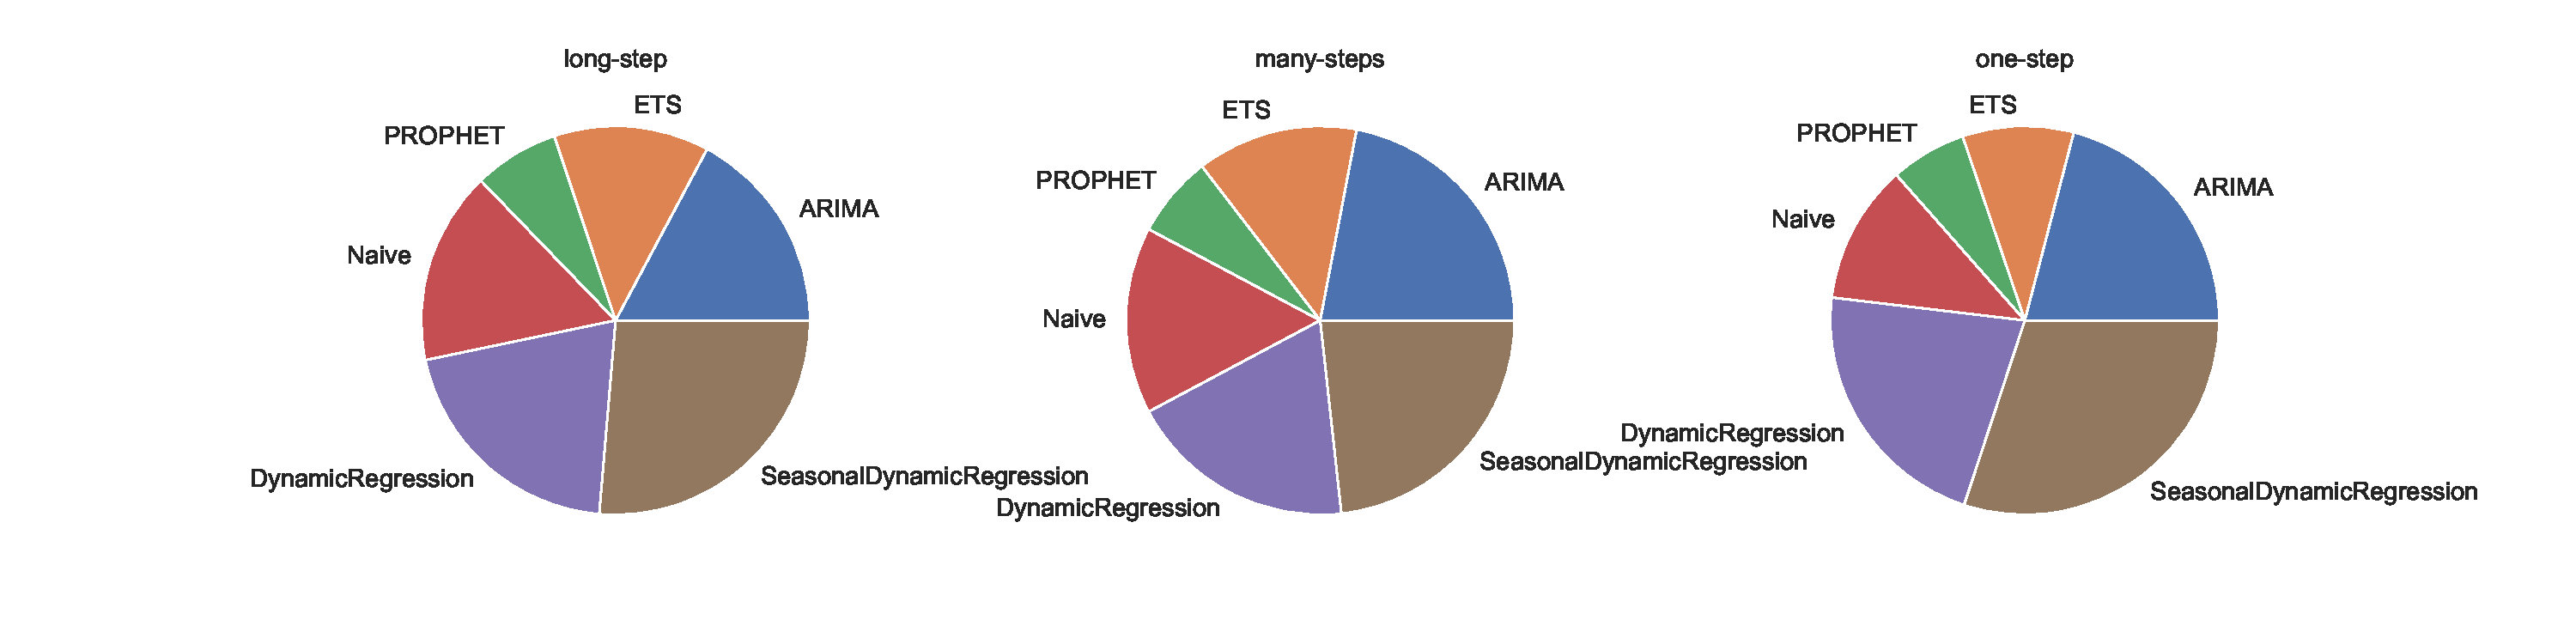
\includegraphics[width=\linewidth]{pictures/wins-fh.pdf}
		\caption{Проценты побед рассматриваемых моделей в зависимости от горизонта прогнозирования}
		\label{wins:fh}
	\end{figure}

	Таким образом, динамические модели действительно можно признать достаточно сильными. Однако необходимо сказать, что здесь есть некоторый сдвиг, заключающийся в том, что в эксперименте более тщательно проводился подбор гиперпараметров для динамических моделей, чем для базовых методов. Таким образом, у динамических моделей изначально было некоторое преимущество. Основные факторы, которые могут влиять на качество их работы --- это периодичность графика, его сезонность и горизонт прогнозирования.
\section{Заключение}
В завершение работы можно ещё раз подчеркнуть, что динамические модели способны показывать достаточно сильное качество и уверенно обходить базовые методы, которые были представлены в данной статье. Также были выявлены оптимальные свойства рядов для прогнозирования с помощью динамических моделей: в идеале ряд должен быть дневным, квартальным или годовым, он должен быть сезонным, а также горизонт прогнозирования не должен включать в себя большой путь. 

Из направления дальнейшей работы можно указать реализацию более эффективного способа оценки параметров, например, L-BFGS; можно добавить в модель экзогенные переменные; поработать над качеством кода, в том числе провести дополнительный рефакторинг и добавить юнит-тесты; добавить сравнение с методами из машинного обучения, например, с градиентным бустингом. 

\newpage 

\begin{thebibliography}{99}
	\bibitem{hartley72}\hypertarget{hartley72}{}
	\href{https://www.jstor.org/stable/2525851}
	{Hartley, M. J. Optimum Simulation Path Estimators. In International Economic Review (1972).}
	\bibitem{calzolari87}\hypertarget{calzolari87}{}
	\href{https://www.jstor.org/stable/1913569}
	{Calzolari, G. Forecast Variance in Dynamic Simulation of Simultaneous Equation Models. In Econometrica (1987).}
	\bibitem{gandrud15}\hypertarget{gandrud15}{}
	\href{https://mran.microsoft.com/snapshot/2015-11-17/web/packages/dynsim/vignettes/dynsim-overview.pdf}
	{Gandrud, C., Williams, L. K., \& Whitten, G. D. Dynamic Simulations of Autoregressive Relationships in R with dynsim. (2015).}
	\bibitem{williams11}\hypertarget{williams11}{}
	\href{http://web.missouri.edu/~williamslaro/Dynamic%20Simulations--Stata%20Journal.pdf}
	{Williams, L. K., Whitten, G. D. Dynamic Simulations of Autoregressive Relationships. In The Stata Journal (2011).}
	\bibitem{johnston74}\hypertarget{johnston74}{}
	\href{https://link.springer.com/chapter/10.1007/978-1-349-01936-6_2}
	{Johnston, H. N., Klein, L., \& Shinjo, K. Estimation and Prediction in Dynamic Econometric Models. In Essays in honor of Jan Tinbergen (1974). London: Macmillan.}
	\bibitem{brown56}\hypertarget{brown56}{}
	\href{http://legacy.library.ucsf.edu/tid/dae94e00;jsessionid=104A0CEFFA31ADC2FA5E0558F69B3E1D.tobacco03}
	{Brown R. G. Exponential Smoothing for Predicting Demand. (1956).}
	\bibitem{holt57}\hypertarget{holt57}{}
	{Holt C. C. Forecasting Trends and Seasonal by Exponentially Weighted Averages. In Office of Naval Research Memorandum (1957).}
	\bibitem{box70}\hypertarget{box70}{}
	\href{https://books.google.ru/books?hl=en&lr=&id=rNt5CgAAQBAJ&oi=fnd&pg=PR7&dq=Box+Jenkins+time+series+analysis+forecasting+and+control&ots=DK52vUm_Vz&sig=niRC2Tt2tUbjb6GQVpyfw2huG6U&redir_esc=y#v=onepage&q=Box%20Jenkins%20time%20series%20analysis%20forecasting%20and%20control&f=false}
	{Box, G., Jenkins, G. Time Series Analysis: Forecasting and Control. In San Francisco: Holden-Day (1970).}
	\bibitem{taylor17}\hypertarget{taylor17}{}
	\href{https://peerj.com/preprints/3190/}
	{Taylor, S. J, Letham, B. Forecasting at Scale. In PeerJ Preprints (2017).}
	\bibitem{cleveland90}\hypertarget{cleveland90}{}
	\href{http://www.nniiem.ru/file/news/2016/stl-statistical-model.pdf}
	{Cleveland, R. B., Cleveland, W. S, McRae, J. E., Terpenning, I. STL: A Seasonal-Trend Decomposition Procedure Based on LOESS. In Journal of Official Statistics (1990).}
	\bibitem{kwiatkowski92}\hypertarget{kwiatkowski92}{}
	\href{https://doi.org/10.1016%2F0304-4076%2892%2990104-Y}
	{Kwiatkowski, D., Phillips, P. C. B., Schmidt, P., Shin, Y. Testing the null hypothesis of stationarity against the alternative of a unit root. In Journal of Econometrics (1992).}
\end{thebibliography}
	
\end{document}
